% ------------------------------------------------------------------------
% ------------------------------------------------------------------------
% abnTeX2: Modelo de Trabalho Academico (tese de doutorado, dissertacao de
% mestrado e trabalhos monograficos em geral) em conformidade com 
% ABNT NBR 14724:2011: Informacao e documentacao - Trabalhos academicos -
% Apresentacao
%
% Adaptado por Emerson Ribeiro de Mello (2017-08-23)
% baseado no modelo "Template para elaboração de trabalho acadêmico - versão setembro/2016" fornecido pela Biblioteca do IFSC - http://www.ifsc.edu.br/menu-colecao-abnt (acessado em 2017-08-23)
% ------------------------------------------------------------------------
% ------------------------------------------------------------------------
\documentclass[
	% -- opções da classe memoir --
	10pt,				% tamanho da fonte
	openright,			% capítulos começam em pág ímpar (insere página vazia caso preciso)
	twoside,			% para impressão em verso e anverso. Oposto a oneside
	a4paper,			% tamanho do papel. 
	% -- opções da classe abntex2 --
	chapter=TITLE,		% títulos de capítulos convertidos em letras maiúsculas
	%section=TITLE,		% títulos de seções convertidos em letras maiúsculas
	%subsection=TITLE,	% títulos de subseções convertidos em letras maiúsculas
	%subsubsection=TITLE,% títulos de subsubseções convertidos em letras maiúsculas
	% -- opções do pacote babel --
	english,			% idioma adicional para hifenização
%	french,				% idioma adicional para hifenização
%	spanish,			% idioma adicional para hifenização
	brazil				% o último idioma é o principal do documento
	]{abntex2}

%	Todas as indicações de pacotes e configurações estão no arquivo de estilo
%  chamado estilo-monografia-ifsc.sty.
\usepackage{estilo-monografia-ifsc}	
\usepackage{xcolor}
\newcommand\adESS[1]{\textcolor{red}{#1}}
%---------------------------------------------------------------------%
%---------------------------------------------------------------------%
% Informações de dados para CAPA e FOLHA DE ROSTO
%---------------------------------------------------------------------%
%---------------------------------------------------------------------%
\titulo{Provimento de QoS para Aplicações em Redes de Sensores\\ sem Fios Baseadas em Redes Definidas por Software}
\autor{André Felippe Weber}
\local{São José - SC}
\data{agosto/2017}
\orientador{Prof. Tiago Semprebom, Dr. Eng.}
\coorientador{Prof. Eraldo Silveira e Silva, Dr. Eng.}
\instituicao{%
  Instituto Federal de Santa Catarina -- IFSC
  \par
  Campus São José
  \par
  Engenharia de Telecomunicações}
\tipotrabalho{Monografia (Graduação)}

% O preambulo deve conter o tipo do trabalho, o objetivo, 
% o nome da instituição e a área de concentração 
\preambulo{Trabalho de conclusão de curso apresentado à Coordenadoria do Curso de Engenharia de Telecomunicações do campus São José do Instituto Federal de Santa Catarina para a obtenção do diploma de Engenheiro de Telecomunicações.}
%---------------------------------------------------------------------%
\textoaprovacao{Este trabalho foi julgado adequado para obtenção do título de Engenheiro de Telecomunicações, pelo Instituto Federal de Educação, Ciência e Tecnologia de Santa Catarina, e aprovado na sua forma final pela comissão avaliadora abaixo indicada.}





%---------------------------------------------------------------------%
% Início do documento
%---------------------------------------------------------------------%


\begin{document}
% Seleciona o idioma do documento (conforme pacotes do babel)
\selectlanguage{brazil}
% Retira espaço extra obsoleto entre as frases.
\frenchspacing 


% ----------------------------------------------------------
% ELEMENTOS PRÉ-TEXTUAIS
% ----------------------------------------------------------
% \pretextual

\imprimircapa
% Folha de rosto - (o * indica que haverá a ficha bibliográfica)
\imprimirfolhaderosto*
% ---

%---------------------------------------------------------------------%
% RESUMOS
%---------------------------------------------------------------------%
% resumo em português
\setlength{\absparsep}{18pt} % ajusta o espaçamento dos parágrafos do resumo
\begin{resumo}
 
As Redes de Sensores sem Fios (RSSFs) tornaram-se um recurso valioso no contexto da Internet das Coisas (IoT). Diversos domínios de aplicação como militar, hospitalar, de segurança e de sistemas de controle utilizam dados escalares e multimídia, produzidos por inúmeros módulos espalhados em uma região. As limitações de bateria, poder de processamento e memória, em conjunto com a heterogeneidade dos módulos utilizados, resultam em um complexo processo de gerenciamento da rede. Como consequência, atender aos requisitos de QoS (\textit{Quality of Service}), aliados ao baixo consumo energético e roteamento eficiente de dados nas RSSFs torna-se um desafio. O conceito de Redes Definidas por Software (SDN), possibilita minimizar a complexidade de gerenciamento dessas redes ao centralizar as decisões de roteamento e administração da RSSF em um controlador separa, fisicamente, da rede. Deste modo, este trabalho propõe implementar uma RSSF baseada no conceito de SDN, que utiliza a plataforma SDN-WISE para prover QoS, através da alocação de largura de banda e economia energética dos módulos, às aplicações que executam sobre a RSSF.

\textbf{Palavras-chave}: Redes de Sensores Multimídia sem Fios, roteamento, QoS, IoT, SDN.

\end{resumo}

%---------------------------------------------------------------------%
% inserir lista de ilustrações, tabelas, listagem de códigos, abreviaturas, símbolos
%---------------------------------------------------------------------%
\pdfbookmark[0]{\listfigurename}{lof}
\listoffigures*
\cleardoublepage
% inserir lista de tabelas
%\pdfbookmark[0]{\listtablename}{lot}
%\listoftables*
%\cleardoublepage


% inserir lista de abreviaturas e siglas
\pdfbookmark[0]{Lista de abreviaturas e siglas}{loa}
%%%%%%%%%%%%%% Como usar o pacote acronym
% \ac{acronimo} -- Na primeira vez que for citado o acronimo, o nome completo irá aparecer
%                  seguido do acronimo entre parênteses. Na proxima vez somente o acronimo
%                  irá aparecer. Se usou a opção footnote no pacote, entao o nome por extenso
%                  irá aparecer aparecer no rodapé
%
% \acf{acronimo} -- Para aparecer com nome completo + acronimo
% \acs{acronimo} -- Para aparecer somente o acronimo
% \acl{acronimo} -- Nome por extenso somente, sem o acronimo
% \acp{acronimo} -- igual o \ac mas deixando no plural com S (ingles)
% \acfp{acronimo}--
% \acsp{acronimo}--
% \aclp{acronimo}--

\chapter*{Lista de abreviaturas e siglas}%
% \addcontentsline{toc}{chapter}{Lista de abreviaturas e siglas}
\markboth{Lista de abreviaturas e siglas}{}


\begin{acronym}
    \acro{ADR}{\textit{Adaptive Data Rate}}
    \acro{AES}{\textit{Advanced Encryption Standard}}
	\acro{API}{\textit{application programming interface}}
	\acro{CAP}{Período de Acesso com Contenção}
	\acro{CCA}{\textit{Clear Channel Assessment}}
    \acro{CE}{\textit{Control Element}}
	\acro{CFP}{Período de Acesso sem Contenção}
    \acro{CSMA}{\textit{Carrier Sense Multiple Access}}
	\acro{CS-MA/CA}{\textit{Carrier Sense Multiple Access with Collision Avoidance}}
    \acro{CSS}{\textit{chirp spread spectrum}}
	\acro{CTS}{\textit{Clear to Send}}
    \acro{DPID}{\textit{Datapath Identifier}}
	\acro{ED}{\textit{Energy Detection}}
	\acro{XML}{\textit{Extensible Markup Language}}
    \acro{FE}{\textit{Forwarding Element}}
	\acro{FFD}{Dispositivo de Função Completa}
    \acro{ForCES}{\textit{Forwarding and Control Element Separation}}
	\acro{FWD}{Forwarding}
	\acro{GTS}{Compartimento de Tempo Garantido}
    \acro{ID}{identificação}
    \acro{IEEE}{\textit{Institute of Electrical and Electronics Engineers}}
    \acro{IETF}{\textit{Internet Engineering Task Force}}
    \acro{IFSC/SJ}{Instituto Federal de Santa Catarina - Câmpus São José}
	\acro{INPP}{\textit{In-Network Packet Processing}}
	\acro{IoT}{Internet das Coisas}
    \acro{IP}{\textit{Internet Protocol address}}
	\acro{ISM}{Industrial, Cientifico e Médico}
	\acro{LFB}{\textit{Logical Function Block}}
	\acro{LPWAN}{\textit{Low Power Wide Area Network}}
	\acro{LQI}{\textit{Link Quality Indication}}
	\acro{LR-WPAN}{\textit{Low-Rate Wireless Personal Area Network}}
	\acro{MAC}{Controle de Acesso ao Meio}
	\acro{MANET}{Rede \textit{Ad hoc} móvel}
	\acro{PAN}{\textit{Personal Area Network}}
	\acro{PHY}{física}
	\acro{QoS}{Quality of Service}
	\acro{RAM}{\textit{Random Access Memory}}
	\acro{RFD}{Dispositivo de Função Reduzida}
	\acro{ROM}{\textit{Read Only Memory}}
	\acro{RSMSF}{Rede de Sensores Multimídia sem Fio}
	\acro{RSSF}{Rede de Sensores Sem Fio}
	\acro{RSSI}{\textit{Received signal strength indication}}
	\acro{RTS}{\textit{Request to Send}}
	\acro{SDN}{Redes Definidas por Software}
	\acro{SDN-WISE}{\textit{Software Defined Networking for WIreless SEnsor networks}}
	\acro{SNR}{relação sinal-ruído}
	\acro{TCP}{\textit{Transmission Control Protocol}}
	\acro{TD}{\textit{Topology Discovery}}
	\acro{TTL}{\textit{Time To Live}}
\end{acronym}


\cleardoublepage

%---------------------------------------------------------------------%

%---------------------------------------------------------------------%
% inserir o sumario
%---------------------------------------------------------------------%
\pdfbookmark[0]{\contentsname}{toc}
\tableofcontents*
\cleardoublepage

% ----------------------------------------------------------
% ELEMENTOS TEXTUAIS
% ----------------------------------------------------------
\textual


% ----------------------------------------------------------
% Inclusão dos capítulos que estão em outros arquivos .tex
% ----------------------------------------------------------
% ----------------------------------------------------------------------- %
% Arquivo: cap1.tex
% ----------------------------------------------------------------------- %
\chapter{Introdução}
\label{c_introducao}

O conceito de \ac{IoT} tem sido amplamente investigado pela comunidade acadêmica nos últimos anos e atualmente ganha espaço nos setores de desenvolvimento das empresas de tecnologia. De acordo com o conceito de \ac{IoT} objetos comuns do cotidiano, como lâmpadas e sensores são conectados à Internet, permitindo, por exemplo, o controle de eletrodomésticos e a disponibilização de dados como umidade e temperatura de ambientes na Internet. 

As aplicações de sensoriamento na \ac{IoT} possuem o desafio de organizar uma rede com centenas de dispositivos. Por isso, as \ac{RSSF} são um recurso valioso da \ac{IoT} \cite{Capella}. As \ac{RSSF}s tendem a executar uma função colaborativa onde os sensores proveem dados, que são processados (ou consumidos) por módulos especiais chamados de sorvedouros (\textit{sink nodes}). Estes módulos sensores geram dados escalares (pressão, temperatura, umidade, etc) e multimídia através de suas câmeras, microfones e sensores. Transmitem essas grandezas utilizando transceptores acoplados aos módulos, e são limitados em memória, processamento e bateria.

Com a popularização da \ac{IoT}, as dificuldades relacionadas à manutenção das aplicações e do roteamento das \ac{RSSF} ficaram ainda mais latentes, principalmente, devido às limitações de \textit{hardware} dos módulos (i.e. processamento, memória e bateria). Dessa forma, existe a demanda no desenvolvimento de técnicas de gerenciamento que melhorem a escalabilidade das RSSFs. O conceito de Redes Definidas por Software (\ac{SDN}) surge como uma das técnicas utilizadas nas \ac{RSSF}s para gerenciamento da topologia, consumo energético e roteamento da rede para satisfazer às exigências de largura de banda e eficiência energética das aplicações \cite{Ndiaye}.

O principio básico da \ac{SDN} é a separação da rede em plano de controle e plano de dados. Onde o primeiro é responsável pelas decisões de roteamento e o segundo pelo encaminhamento dos dados. Dessa forma, um controlador centralizado, em um servidor remoto, controla e gerencia o encaminhamento realizado pelos módulos no plano de dados. Por exemplo, um controlador de uma \ac{RSSF} em uma \textit{Smart Home} pode utilizar algoritmos complexos de roteamento para garantir, em tempo real, a banda necessária para que um sensor com capacidade multimídia transmita seus dados, de acordo com as demandas de \ac{QoS} (\textit{Quality of Service}) da aplicação. 

O protocolo \ac{SDN-WISE} se baseia na arquitetura \ac{SDN} para reduzir a complexidade de configuração e gerenciamento das \ac{RSSF}s. Desta forma, um controlador separado fisicamente do restante da rede executa algoritmos de roteamento complexos em um servidor remoto, enquanto módulos da rede encaminham os dados de um nó \textit{source} até o \textit{sink}, de acordo com a tabela de roteamento recebida do controlador.

A utilização da abordagem \ac{SDN} economiza energia dos módulos e permite o uso de algoritmos complexos de roteamento que visam a garantia de \ac{QoS} para as aplicações da rede. Deste modo, este trabalho propõe um sistema que utiliza o protocolo \ac{SDN-WISE} para capturar informações do estado dos enlaces da \ac{RSSF} e enviar para um controlador remoto (na nuvem), que executa um algoritmo de roteamento. A Figura \ref{modeloDoSistema} ilustra uma \ac{RSSF} que, pode usufruir do sistema proposto. Os módulos da \ac{RSSF} enviam, através do protocolo \ac{SDN-WISE}, informações como qualidade do enlace e, nível de bateria para um controlador da rede, hospedado na nuvem. O controlador, por sua vez, executa um algoritmo de roteamento que, prioriza uma métrica de \ac{QoS} da aplicação em sua execução. Por exemplo, maximização do tempo de vida da rede ou largura de banda. Por fim, após a execução do algoritmo, o controlador envia uma mensagem de atualização para os módulos da rede que, podem alterar ou adicionar novas rotas de encaminhamento de mensagens.

\begin{figure}[h!]
    \centering
    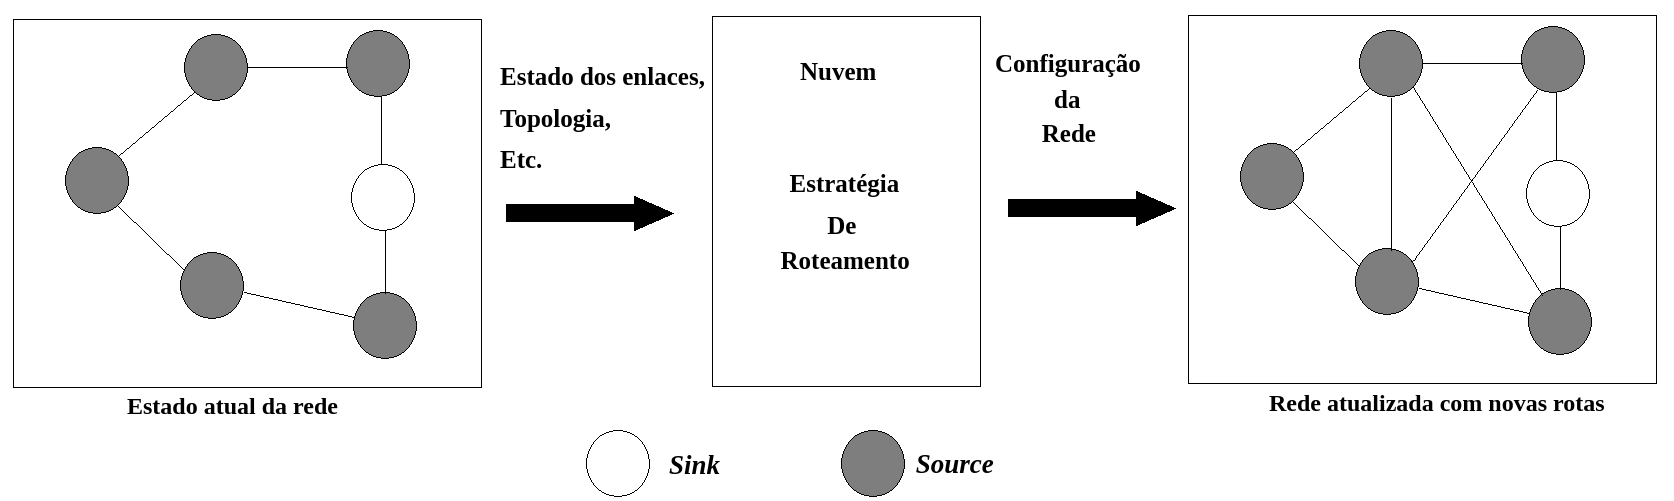
\includegraphics[width=15cm]{figs/overviewDoSistema.png}
    \caption{Modelo do sistema.}
    \label{modeloDoSistema}
\end{figure}

\section{Objetivos Gerais}
\label{s_introducao_OG}

O objetivo geral deste trabalho é implementar uma rede de sensores sem fio, baseada no conceito de Redes Definidas por Software (SDN) com fins de atender aos requisitos de \ac{QoS} das aplicações que se executam sobre a \ac{RSSF}.

\section{Objetivos específicos}
\label{s_introducao_OE}
\begin{itemize}
  \item Implantar e analisar o comportamento de uma aplicação sobre a plataforma \ac{SDN-WISE} no simulador Cooja e nos sensores Micaz;
  \item Conceber e implementar um controlador \ac{SDN} que possibilite construir regras de roteamento a partir de uma configuração estática dos módulos e, dos fluxos que possuem requisitos de \ac{QoS} associados à largura de banda e ao nível de bateria dos módulos;
  \item Implantar uma rede real com a aplicação definida anteriormente e avaliar o comportamento da mesma.
  \item Analisar algoritmos de roteamento para \ac{RSSF} e, adequá-los para o cumprimento de requisitos de \ac{QoS} referentes à vazão e consumo energético das aplicações que executam sobre o \ac{SDN-WISE};
  \item Implementar as regras de roteamento em uma aplicação piloto, utilizando o simulador Cooja.
\end{itemize}
 % introdução
% ----------------------------------------------------------------------- %
% Arquivo: cap2.tex
% ----------------------------------------------------------------------- %

\chapter{Fundamentação Teórica}
\label{c_cap2}

Neste capítulo serão apresentados temas essenciais para a compreensão e desenvolvimento deste trabalho. Na Seção \ref{s_c2_IoT} é explicado como as \ac{RSSF}s são utilizadas para dar forma à muitas aplicações de sensoriamento da \ac{IoT}. Na Seção \ref{s_c2_sdn} é apresentado o conceito de \ac{SDN} e como tais redes são empregadas. Na sequência, Seção \ref{s_c2_wise_sdn},  o conceito de \ac{SDN} é explorado no contexto de \ac{RSSF}s. Para tanto, a  plataforma \ac{SDN-WISE} será usada como referência, através de um exemplo. Finalmente, a aplicabilidade desta plataforma em aplicações com requisitos de \ac{QoS} é discutida.

\section{Redes de Sensores para a Internet das Coisas}
\label{s_c2_IoT}

A \ac{IoT} considera que os objetos comuns do cotidiano se comuniquem através da Internet. Esta ideia já pode ser observada na prática nos dispositivos inteligentes, como televisores, celulares e relógios além de outros objetos, como lâmpadas e sensores. Porém, o aumento do número de dispositivos conectados à Internet impõe o desafio de rotear, de maneira eficaz, o volume de dados gerados que cresce proporcionalmente. 

O desafio de organizar uma rede com centenas de dispositivos é uma realidade, principalmente quando se trata de aplicações de sensoriamento. Por isso, as \ac{RSSF}s são um recurso valioso da \ac{IoT} \cite{Capella}. Criadas na década de 1950, as \ac{RSSF}s foram, no princípio, utilizadas pelo exército norte americano
para detectar a movimentação de submarinos soviéticos \cite{Nasir}. Com o avanço tecnológico elas passaram a ser implementadas em zonas terrestres e subterrâneas, além das subaquáticas. Dentre as aplicações mais citadas em publicações atuais estão aquelas que abrangem a área da saúde, de controle de tráfego de veículos, monitoramento e militar. 

As \ac{RSSF} atuais são compostas por diversos módulos equipados com processador, memórias \ac{ROM} e \ac{RAM}, rádio transceptor, um ou mais sensores e uma fonte de energia. Algumas redes utilizam estações base com melhor poder de processamento e capacidade energética para receber e tratar os dados gerados pelos módulos. Dessa forma, é necessário garantir que os módulos comuniquem-se entre si e com a estação base, mesmo que indiretamente, a fim de realizar a entrega de pacotes a qualquer destinatário da rede e garantir que as exigências de \ac{QoS} sejam cumpridas \cite{Guy}.

O conjunto de métricas de performance utilizadas para definir a qualidade do serviço nas \ac{RSSF}s variam de acordo com a necessidade de cada aplicação. Porém, segundo \citeonline{Nasir}, existem oito métricas que são comumente utilizadas: (I) vazão, (II) atraso fim-a-fim, (III) taxa de sucesso na entrega de pacotes, (IV) perda de pacotes, (V) distância medida através da quantidade de saltos (\textit{hops}) entre a fonte e o destinatário, (VI) consumo e eficiência energética, (VII) carga da rede e (VIII) longevidade.

A topologia de rede comumente utilizada para organizar as \ac{RSSF}s é a Ponto-a-Ponto. Como mostrado na Figura \ref{TopologiaPontoAPonto}, a comunicação das redes ponto-a-ponto é, normalmente, realizada entre os vizinhos mais próximos. Os integrantes da rede podem atuar como fonte, receptor ou roteador dos dados já que para realizar a comunicação com um destino fora de alcance é necessário rotear os dados através dos vizinhos. Devido às limitações de processamento e de consumo de energia dos módulos a comunicação entre vizinhos é a principal razão para o uso desta topologia nas \ac{RSSF}s. 

\begin{figure}[!htb]
    \centering
    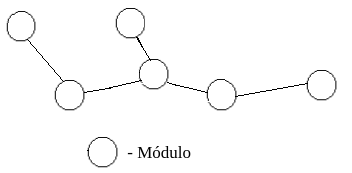
\includegraphics[width=8cm]{figs/redepontoaponto.png}
    \caption{Topologia ponto-a-ponto.}
    \label{TopologiaPontoAPonto}
\end{figure}


Atualmente, verifica-se que parte da atenção destinada ao estudo das \ac{RSSF}s é dirigida ao estudo de redes de sensores com capacidade de processar dados multimídia. Isto se deve ao avanço tecnológico e à redução do custos de aquisição dos módulos e outros componentes utilizados nas \ac{RSMSF}s. As \ac{RSMSF}s são compostas por módulos equipados com câmeras, microfones e outros sensores produtores de conteúdo multimídia \cite{Shakshuki}, além de módulos equipados somente com transceptores utilizados no roteamento de dados na rede. 

As \ac{RSMSF}s atraíram atenção dos pesquisadores da área devido ao seu potencial científico e aplicações atrativas \cite{Shen}. Por exemplo, a distribuição de câmeras ao longo de uma rodovia assegura a redundância do sistema de videomonitoramento, disponibiliza múltiplos pontos de vista e, através da escolha de câmeras mais próxima ou com qualidade superior, amplia o ângulo de visão de um evento. A adição de microfones ao sistema permite detectar e determinar a localização aproximada de sons incomuns ao ambiente como barulhos de tiros \cite{Ang} ou freadas bruscas.

%Dentre as aplicações mais citadas em publicações atuais estão aquelas na área militar, da saúde, de controle de tráfego de veículos, monitoramento e vigilância. Aplicações que compreendem esta última área são utilizadas principalmente quando a complexidade do sistema aumenta devido ao grande número de câmeras espalhadas em espaços públicos como bancos, aeroportos e \textit{shopping centers} \cite{Natarajan}. A ampla cobertura característica de uma rede de sensores multimídia tem como principal vantagem facilitar o rastreamento de suspeitos e a oferta de diferentes ângulos de visão de uma mesma cena. 

Devido ao maior fluxo de dados gerado pelas aplicações implementadas nas \ac{RSMSF}s, em comparação com as \ac{RSSF}s, as métricas de \ac{QoS} que atuam diretamente na garantia de entrega e integridade dos dados multimídia ganham maior relevância em detrimento do consumo de energia que, nas redes \ac{RSSF}s, ocupa o posto de destaque \cite{Zara,Akyildiz}. As exigências de \ac{QoS} nas \ac{RSMSF}s podem variar de uma aplicação para outra. Por exemplo, uma aplicação de controle de fluxo de tráfego é mais tolerante à falhas na entrega de pacotes que uma aplicação militar. Porém, de forma geral, as métricas de \ac{QoS} utilizadas nas redes \ac{RSMSF}s visam a garantia de largura de banda, tempo de vida da rede, controle do \textit{jitter}\footnote{Variação no atraso}, taxas de atraso toleráveis, controle de erro através de técnicas de codificação de fonte de baixa complexidade e estratégias de melhoria da eficiência energética \cite{Zara}.

%Dentre as tecnologias desenvolvidas e implementadas nas \ac{RSSF}s está a \ac{LR-WPAN} que define redes com baixas taxas de dados, baixo consumo energético e baixo custo. O padrão IEEE 802.15.4 (ver \autoref{s_c2_iee802154}) utilizado nas \ac{RSSF}s especifica as camadas \ac{PHY} e de \ac{MAC} e proporciona a criação de redes \ac{LR-WPAN}. Outra tecnologia, mais recente, é o LoRa que também permite criar \ac{LR-WPAN} porém com um alcance maior que o proporcionado pelo IEEE 802.15.4 e com taxas de dados mais baixas.

\subsection{Tecnologias para Redes de Sensores sem Fios}
\label{s_c2_tech}
\subsubsection{IEEE 802.15.4}
Dentre as tecnologias desenvolvidas e implementadas nas \ac{RSSF}s está o padrão IEEE 802.15.4 que
especifica as camadas \ac{PHY} e de \ac{MAC} para redes \ac{LR-WPAN} e, portanto se caracteriza pela comunicação sem fio com baixa taxa de transmissão de dados, baixo consumo energético e custo de implementação. Segundo \citeonline{SEMPREBOM}, apesar de não ter sido projetada especificamente para as \ac{RSSF}s, o IEEE 802.15.4 vem sendo amplamente adotado e possibilitou o surgimento de novos produtos baseados nesta tecnologia. 

Na implementação de uma \ac{RSSF} utilizando a tecnologia IEEE 802.15.4 os módulos podem ser categorizados, de acordo com sua capacidade de processamento ou função na rede, em dois tipos:

\begin{itemize}
  \item \textbf{\ac{FFD}}: Obrigatório em uma \ac{LR-WPAN}, este dispositivo suporta até três modos de operação:
  \begin{enumerate}
     \item \textbf{Coordenador PAN}: O dispositivo fica responsável por controlar a \ac{PAN} e identificar a rede para que outros dispositivos se associem \cite{BONOTTO}. 
     \item \textbf{Coordenador}: Dispositivo que deve, obrigatoriamente, estar associado à um Coordenador \ac{PAN} e oferece o serviço de sincronização através da transmissão de \textit{beacons}.
     \item \textbf{Dispositivo simples}: Dispositivo que atua apenas como um nó na rede e, portanto não implementa as funções de coordenador \ac{PAN} ou coordenador.
  \end{enumerate}
\end{itemize}

\begin{itemize}
  \item \textbf{\ac{RFD}}: Dispositivo associado a um único \ac{FFD} e que opera com implementação miníma do IEEE 802.15.4.
\end{itemize}

No padrão IEEE 802.15.4 é possível utilizar as topologias estrela e ponto-a-ponto. Na topologia estrela existe um único nó central ao qual todos os módulos se conectam, como mostrado na Figura \ref{TopologiaEstrelaSemprebom}. Este dispositivo central deve ser um \ac{FFD} operando como Coordenador \ac{PAN} que fica responsável por iniciar uma nova rede, com um identificador único, e rotear todos os pacotes sendo transmitidos. Os outros integrantes são \ac{RFD}s ou \ac{FFD}s operando como Coordenador ou Dispositivo simples \cite{SEMPREBOM}. 

O nó central da topologia estrela pode ser visto como um ponto crítico de falha, uma vez que toda a comunicação da rede é realizada através dele. Por isso, devido às limitações energéticas dos \ac{FFD}s, o padrão IEEE 802.15.4 recomenda que o Coordenador \ac{PAN} esteja conectado em alguma fonte de alimentação, e que esta topologia seja usada em aplicações que apresentem facilidade na substituição da fonte de energia do Coordenador \ac{PAN}, como automação residencial e industrial  \cite{BONOTTO}.

\begin{figure}[h!]
    \centering
    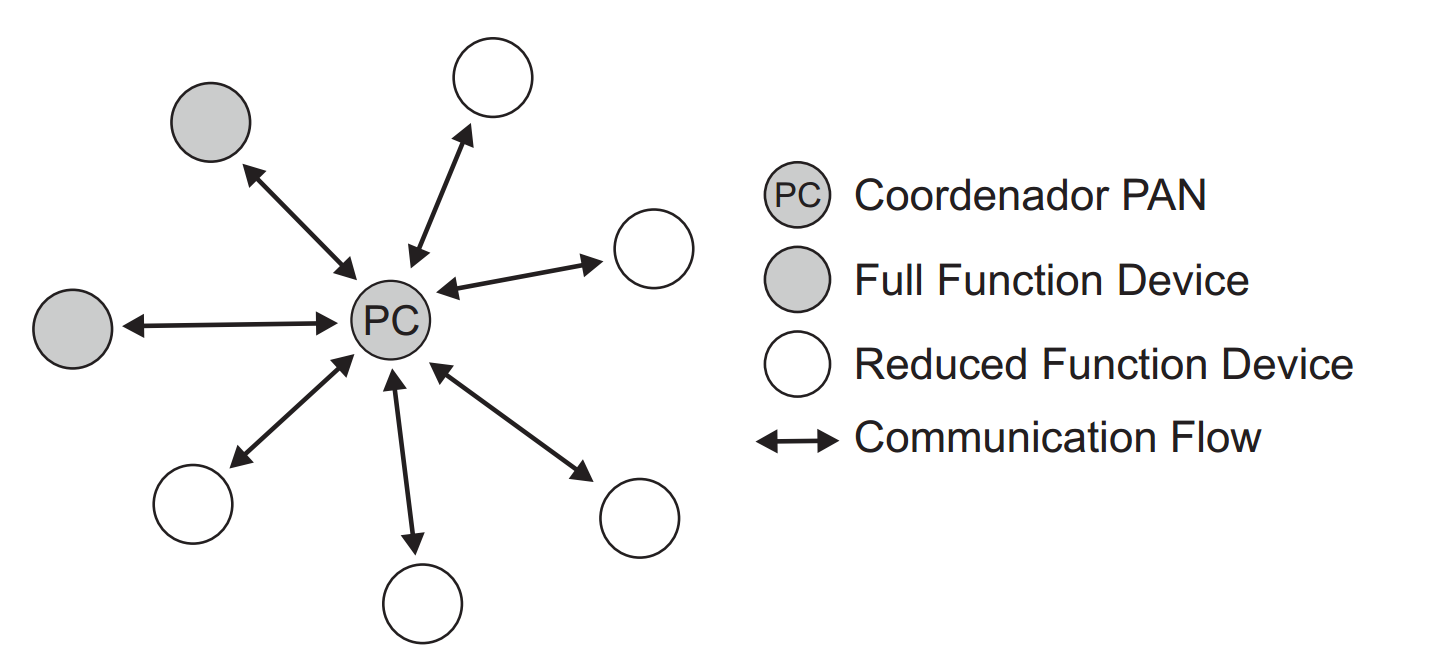
\includegraphics[width=10cm]{figs/TopologiaEstrelaSemprebom.png}
    \caption{Topologia estrela. \cite{SEMPREBOM} }
    \label{TopologiaEstrelaSemprebom}
\end{figure}

A topologia ponto-a-ponto (Figura \ref{TopologiaPontoAPontoSemprebom}), assim como a estrela, possui um único coordenador \ac{PAN}. Porém é mais confiável já que, por ser descentralizada, possui múltiplos caminhos para o roteamento dos pacotes. Por não possuir um nó central, os módulos se comunicam diretamente com os vizinhos em seu raio de cobertura, e através de múltiplos saltos com os vizinhos mais distantes. 

As funcionalidade de roteamento por múltiplos saltos não são definidas pelo padrão IEEE 802.15.4, pois devem ser definidas na camada de rede \cite{SEMPREBOM}. As funções de roteamento utilizadas para realizar os múltiplos saltos possuem a desvantagem de introduzir complexidade e reduzir a longevidade da rede, uma vez que os módulos precisam reencaminhar dados recebidos dos vizinhos. Porém, tem como vantagem o aumento do alcance da rede. 
\newpage
\begin{figure}[h!]
    \centering
    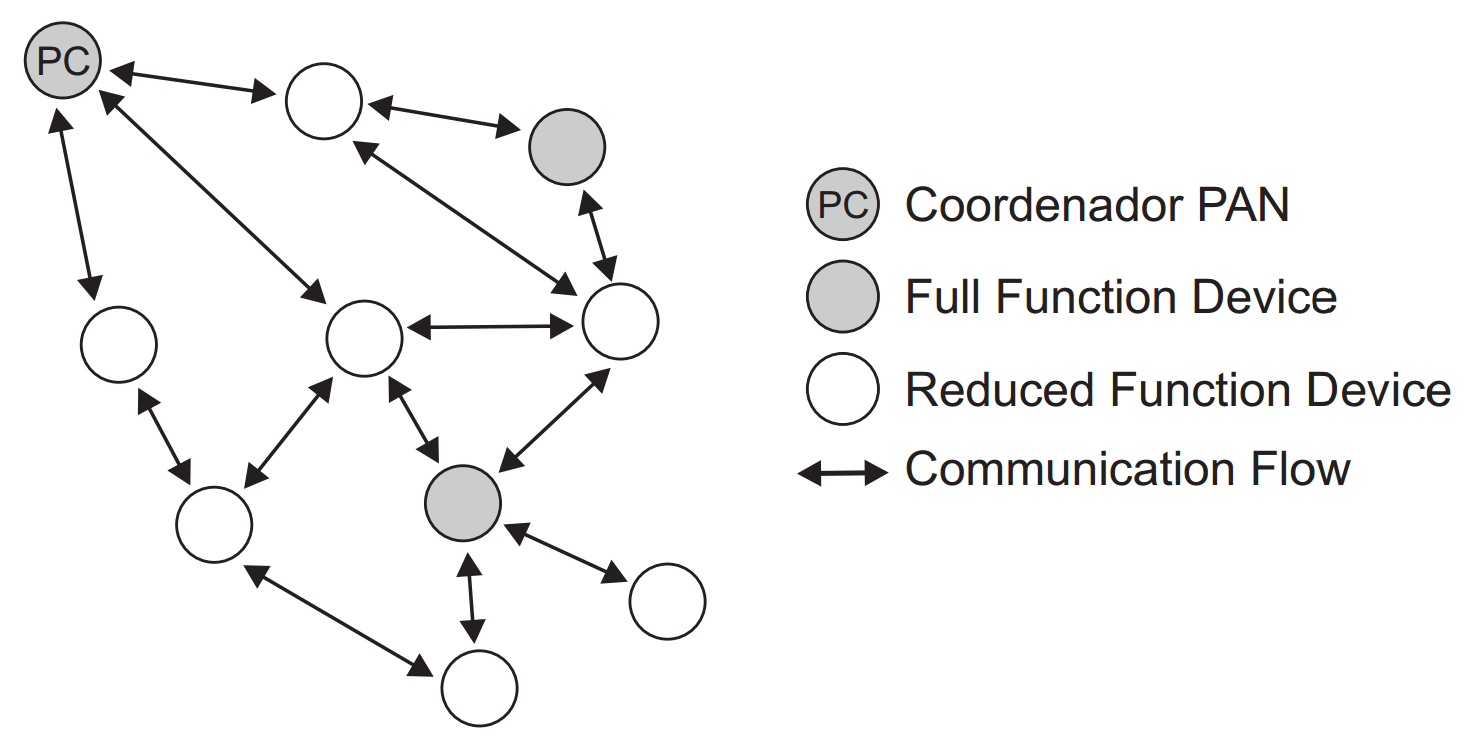
\includegraphics[width=10cm]{figs/TopologiaPontoAPontoSemprebom.png}
    \caption{Topologia ponto-a-ponto \cite{SEMPREBOM}}
    \label{TopologiaPontoAPontoSemprebom}
\end{figure}

%Outra tecnologia que se destaca na criação de \ac{RSSF}s é o LoRa. Esta é uma tecnologia de camada física e uma modulação para comunicação sem fio que possibilita enlaces de longa distância e baixo consumo energético. A técnica de modulação por espalhamento espectral \ac{CSS} foi utilizada por décadas na comunicação militar e espacial devido às suas característica de longo alcance e resistências de interferências. A adoção do \ac{CSS} pelo LoRa permitiu a sua primeira implementação de baixo custo para uso comercial \cite{loraAllianceWhatIs}.

%Na \ac{CSS} um simbolo é codificado em uma sequência maior de bits de forma a aumentar a sensibilidade do receptor, e portanto reduzir a \ac{SNR} necessária para a correta recepção, sem alterar a largura de banda do sinal sem fio. O comprimento do código de espalhamento é variável de acordo com a aplicação em uso no LoRa. Como consequência, é possível variar as taxas de transmissão de dados e melhorar o alcance, resistência à interferências ou o consumo energético \cite{CVZZ16}.

%Segundo \citeonline{LEONAN} isso ocorre pois quanto menor a taxa de transmissão, maior a duração da mensagem (tempo do sinal no ar) e consequentemente maior a energia de bit, resultando no aumento da qualidade de recepção do sinal (cerca de -150 dBm), proporcionando uma maior cobertura, estimada na ordem de 10 a 15 quilômetros em áreas rurais e 2 a 5 quilômetros em áreas urbanas. A frequência de operação do LoRa varia por região porém, assim como o IEEE 802.15.4 operam na faixa \ac{ISM}, mais especificamente em 2.4 GHz, 868/915 MHz, 433 MHz e 169 MHz. A taxa de transmissão está na ordem de centenas de bits ou dezenas de kilobits por segundo \cite{CVZZ16}.
\subsubsection{LoRa}

Outra tecnologia que se destaca na criação de \ac{RSSF}s é o LoRa. Esta é uma tecnologia de camada física e uma modulação para comunicação sem fio que possibilita enlaces de longa distância, baixo consumo energético e taxa de transmissão. Segundo \citeonline{LEONAN}, quanto menor a taxa de transmissão, maior a duração da mensagem (tempo do sinal no ar) e, consequentemente maior a energia de bit. Como resultado, há o aumento da qualidade de recepção do sinal (cerca de -150 dBm), proporcionando uma maior cobertura, estimada na ordem de 10 a 15 quilômetros em áreas rurais e 2 a 5 quilômetros em áreas urbanas. A frequência de operação do LoRa varia por região porém, assim como o IEEE 802.15.4 operam na faixa \ac{ISM}, mais especificamente em 2.4 GHz, 868/915 MHz, 433 MHz e 169 MHz. A taxa de transmissão está na ordem de centenas de bits ou dezenas de kilobits por segundo \cite{CVZZ16}.

O LoRaWAN define o protocolo de comunicação e a arquitetura do sistema para a rede, enquanto a camada física LoRa possibilita o uso de enlaces de longa distância. Apesar do longo alcance, as redes ponto-a-ponto apresentam a desvantagem do consumo desnecessário de bateria no módulos que atuam como roteadores da rede. Por isso, no LoRaWAN adotou-se a topologia estrela de longa distância. O que permite uma maior economia energética para conexões de longa distância.

As redes LoRaWAN são implementadas com o objetivo de otimizar redes \ac{LPWAN} para aplicações \ac{IoT}. As \ac{LPWAN}s oferecem excelente eficiência energética com expectativa de vida útil maior que dez anos para as baterias, e são pensadas para aplicações que transmitem pequenas quantidades de dados, por grandes distâncias e poucas vezes por hora \cite{loraAllianceWhatIs}.

\begin{figure}[h!]
    \centering
    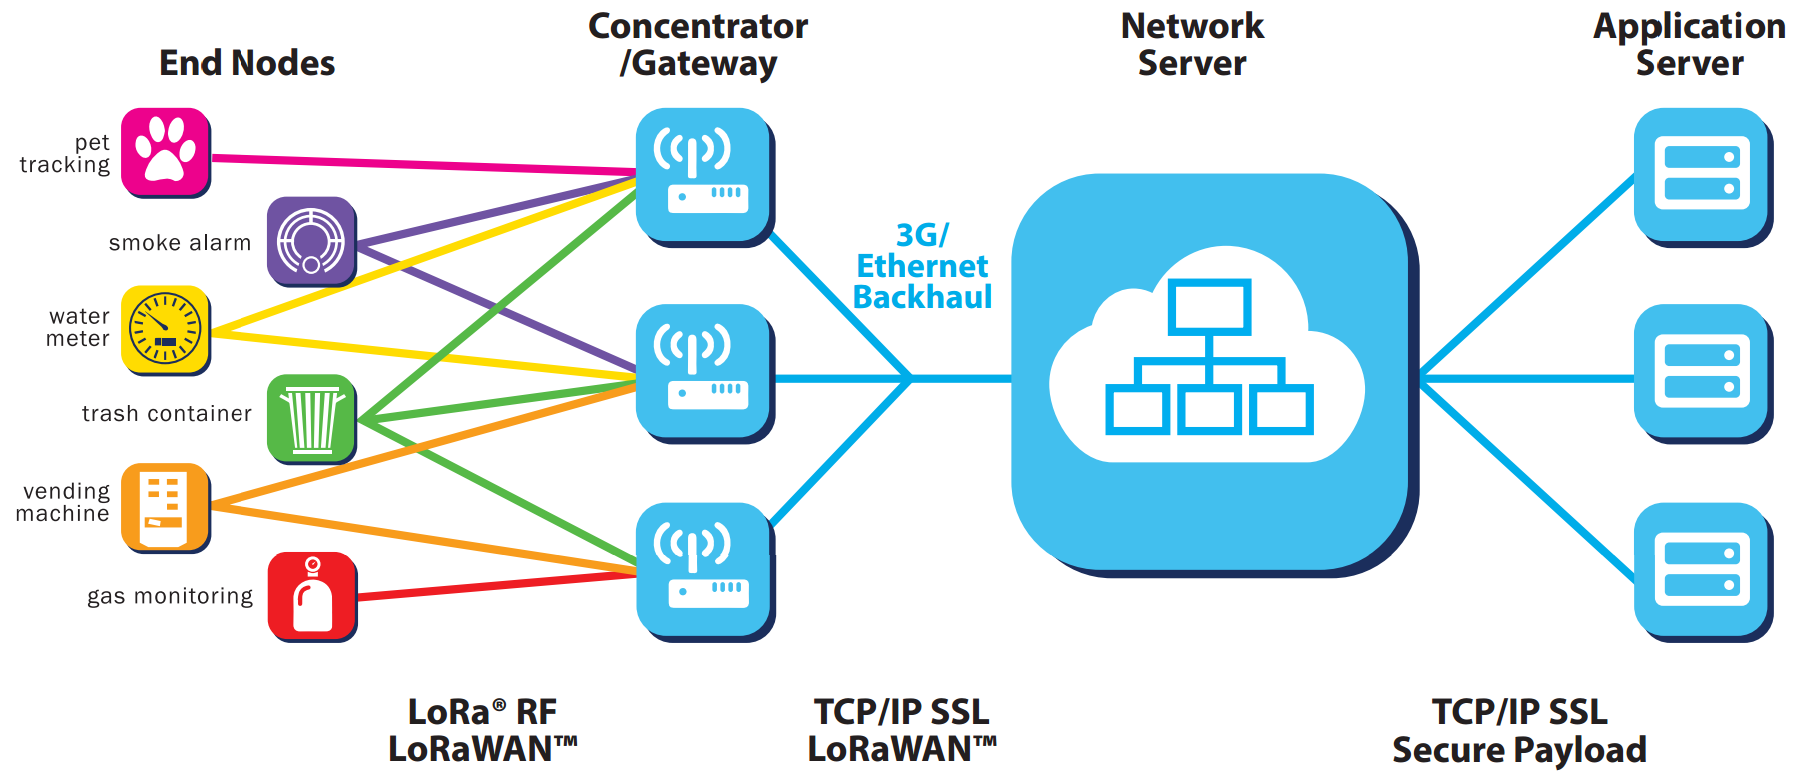
\includegraphics[width=11cm]{figs/LoRaWAN_Overview.png}
    \label{loraWAN_Overview}
    \caption{Visão geral de uma rede LoRaWAN com topologia em estrela \cite{loraAllianceWhatIs}}
\end{figure}

De acordo com \citeonline{loraAllianceWhatIs}, as redes LoRaWAN são compostas por \textit{gateways} que atuam como nó central da rede e módulos (\textit{end-devices}) que compõem a rede. São classificados de acordo com a relação entre disponibilidade de recepção de dados e vida útil de sua bateria:

\begin{itemize}
  \item \textbf{Classe A:} São sensores, energizados via bateria, com a melhor eficiência energética da rede LoRaWAN. Os \textit{end-devices} de classe A transmitem somente quando necessário e recebem dados, apenas, após realizar uma transmissão. Dessa forma, ao realizar uma transmissão o \textit{end-device} espera por duas janelas curtas de tempo e, volta a desabilitar seu rádio transceptor.
  \item \textbf{Classe B:} São atuadores, energizados via bateria, que além de implementar as janelas de recepção do \textit{end-devices} classe A, também agendam janelas de tempo para recepção de dados. Para isso, é necessário a sincronização entre \textit{gateway} e \textit{end-device} classe B que, é realizada através de \textit{beacons} enviados pelo \textit{gateway}.
  \item \textbf{Classe C:} São atuadores conectados à uma fonte externa de energia que, aceitam recepção o tempo todo com exceção para quando há uma transmissão a ser realizada. Esse \textit{end-device} tem a vantagem de eliminar latência para recepção de dados, porém necessita de uma fonte contínua de energia.
\end{itemize}

A topologia em estrela é a ideal para as rede LoRaWAN por causa do longo alcance proporcionado pela camada física dos dispositivos LoRa \cite{GIULIO}. Esta topologia permite uma melhor eficiência energética quando comparada à topologia ponto-a-ponto, adotada nas redes de curto alcance como as redes IEEE 802.15.4, visto que nenhum módulo atua como roteador. E para contornar o ponto de falha único, característico da topologia em estrela, usa-se redundância de \textit{gateways} \cite{loraAllianceWhatIs}. 

Diferentemente do que ocorre na topologia estrela tradicional, em que há apenas um nó central em que todos os módulos de conectam, na LoRaWAN existem diversos nós, implementados como \textit{gateways}. Assim sendo, segundo \citeonline{loraAllianceWhatIs} as mensagens produzidas por um módulo não são recebidas por apenas um, mas sim por múltiplos \textit{gateways}. Cada \textit{gateway} encaminha os dados gerados pelo \textit{end-device} até um servidor responsável por tratar dos dados, eliminar dados redundantes, administrar a taxa de dados, etc. Dessa forma, através da redundância criada por múltiplos \textit{gateways} elimina-se o ponto crítico da rede, que é dispor de um único nó central.

Em \citeonline{loraAllianceWhatIs}, atribuiu-se às redes LoRaWAN a característica de gerenciar a longevidade da bateria, capacidade e segurança da rede, onde:

\begin{itemize}
  \item \textbf{Longevidade da bateria:} Os módulos na LoRaWAN são assíncronos, ou seja, não há troca de mensagem entre \textit{end-devices} ou com o \textit{gateway} para manter sincronia. Logo, ganha-se em eficiência energética, já que o processo de sincronização é o fator número um de redução da vida das baterias \cite{loraAllianceWhatIs}.
  
  \item \textbf{Capacidade da rede:} O LoRaWAN utiliza a sua capacidade de adaptação da taxa de dados (\ac{ADR}) para aumentar a capacidade da rede e que, um \textit{gateway} possui de receber mensagens de um grande volume de \textit{end-devices} \cite{loraAllianceWhatIs}. Isto ocorre pois o uso da \ac{CSS} na camada física permite que um \textit{gateway} receba dados com diferentes taxas de transmissão no mesmo canal e, ao mesmo tempo. Assim, é possível que dispositivos mais próximos do \textit{gateway} operem com uma taxa de transmissão mais alta e, com potência menor que dispositivos mais distantes \cite{LEONAN}.
  
  O \ac{ADR} auxilia, também, no aumento da capacidade da rede já que ele possibilita que seja aumentado a taxa de dados, de forma a reduzir o tempo de transmissão de um módulo e abrindo espaço de tempo para que outros transmitam. Além do mais, é possível reduzir o consumo energético de um módulo ao reduzir sua potência e taxa de dados.
  
  \item \textbf{Segurança da rede:} Na LoRaWAN é utilizado criptografia \ac{AES} e garante-se segurança nas camadas de aplicação e rede. Na camada de aplicação os dados do usuário final são protegidos enquanto na de rede garante-se a autenticidade do módulo \cite{loraAllianceWhatIs}.
\end{itemize}


\subsection{Técnicas de Roteamento em \ac{RSSF}s} 
\label{s_c2_roteamento_RSSF}

Devido às limitações de recursos dos módulos utilizados nas \ac{RSSF}s, é importante projetar protocolos de roteamento que possibilitem a transmissão de pacotes por longas distâncias na rede. Para isso, alguns protocolos utilizam técnicas de múltiplos caminhos e saltos para criar e manter rotas de encaminhamento dos pacotes. Como resultado, o protocolo melhora a eficácia da comunicação entre módulos e em alguns casos, com a Internet.

Muitos protocolos de roteamento para \ac{RSSF}s foram propostos nas últimas décadas considerando as limitações energéticas, de processamento e memória dos módulos, assim como as exigências das aplicações e arquitetura das redes de sensores sem fio \cite{Alazzawi}. Em muitas aplicações de \ac{RSSF}s espera-se que a rede tenha capacidade de organização automática, uma vez que os módulos são distribuídos aleatoriamente e se comportam como componentes de uma rede \textit{ad hoc}. Porém, o roteamento dos dados nas \ac{RSSF}s não pode ser feito como em redes sem fio tradicional. Segundo \citeonline{Singhers}, as \ac{RSSF}s se diferenciam das redes celulares e da \ac{MANET} por possuírem algumas características especiais:

\begin{itemize}
  \item Grandes quantidades de dispositivos na rede. Algumas redes podem ser significantemente mais densamente povoadas que as redes \ac{MANET};
  \item Limitação energética e computacional dos módulos contrastante com o que acontece nas redes sem fio tradicionais;
  \item Auto-organização dos módulos implementada por algumas tecnologias utilizadas nas \ac{RSSF}s, como o Zigbee, que utiliza o padrão IEEE 802.15.4 nas camadas inferiores (\ac{PHY} e \ac{MAC}) e, implementa as camadas superiores introduzindo a capacidade de auto configuração e auto recuperação de falhas;
  \item Os módulos não são confiáveis, uma vez que podem apresentar falha devido às condições ambientais em que são utilizados e por esgotamento da bateria;
  \item Possível redundância na transmissão de dados correlatos devido à proximidade entre módulos equipados com sensores;
  \item Uma \ac{RSSF} é, normalmente, criada para uma aplicação específica visto que as métricas de \ac{QoS} e exigências da rede variam entre aplicações;
  \item A topologia da rede muda constantemente devido à falta de confiabilidade dos módulos, interferências e à possível movimentação dos módulos.
\end{itemize}

%Nos últimos anos diversos estudos foram publicados afim de demonstrar algoritmos de roteamento que abordam características e exigências especificas de uma aplicação na \ac{RSSF}. Por isso, em \citeonline{Singhers} e \citeonline{Tripathy} foram definidas categorias de protocolos, utilizados nas \ac{RSSF}s, de acordo com a localização, mobilidade e capacidade energética dos módulos, hierarquia na rede, roteamento baseado nas métricas de \ac{QoS} e capacidade de roteamento por múltiplos caminhos e saltos. Neste trabalho serão abordados os protocolos que se enquadram nas três últimas categoria citadas. 

Tradicionalmente, protocolos de roteamento utilizam a abordagem \textit{single-path} para escolha de caminhos. Ou seja, baseado em uma métrica de performance ou na menor distância, um único caminho é escolhido. Porém, através da abordagem de roteamento por múltiplos caminhos é possível melhorar a resiliência da rede, ou seja, a capacidade que a rede possui de se recuperar de falhas, visto que protocolos que utilizam a abordagem \textit{single-path} interrompem o roteamento por algum tempo ou por completo em um evento de falha. Segundo \citeonline{Jamal}, o preço que se paga ao melhorar a resiliência da rede é o aumento de tráfego e consumo energético na rede, visto que mensagens periódicas serão transmitidas para manter os caminhos ativos e atualizados. 

Diferentes abordagens podem ser utilizadas para projetar um algoritmo que faz uso de roteamento por múltiplos caminhos. Isso ocorre, pois pode-se priorizar a eficiência energética, ou a confiabilidade da rede, por exemplo. Assim, é possível optar por evitar rotear pacotes por módulos que estão com baixo nível de bateria, dividir um pacote por múltiplos caminhos ou enviar o mesmo pacote por diversos caminhos. Porém, todos os protocolos de roteamento por múltiplos caminhos compartilham três etapas básicas: Descoberta, seleção e manutenção dos caminhos \cite{radi2012multipath}.

Quanto à descoberta dos caminhos, os protocolos podem ser divididos em três categorias de acordo com o grau de separação dos caminhos (\textit{disjointedness}).

\begin{itemize}
  \item \textbf{\textit{Node-disjoint}:} Os caminhos escolhidos não possuem nenhum módulo em comum, além do \textit{source} e \textit{sink}. Ou seja, são completamente independentes um dos outros. Esse tipo de caminhos possuem a desvantagem de apresentar pontos de falha em caso de perda de comunicação em um dos enlaces entre módulos. Por exemplo, na Figura \ref{Node-disjoint}, é possível observar que em caso de falha do módulo C, módulo B também não consegue mais transmitir seus pacotes para o \textit{sink} F. 
  \item \textbf{\textit{Link-disjoint}:} Os caminhos possuem módulos em comum, porém não compartilham os enlaces, como mostrados na Figura \ref{Link-disjoint}. 
  \item \textbf{\textit{partially-disjoint}:} Os caminhos compartilham seus módulos e enlaces. Possui a principal desvantagem de ser vulnerável às falhas desses componentes da rede. Porém, é possível criar diversos caminhos, redundantes, que melhoram a resiliência da rede \cite{radi2012multipath}. 
\end{itemize}

\begin{figure*}[t!]
    \centering
    \begin{subfigure}[t]{0.5\textwidth}
        \centering
        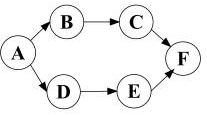
\includegraphics[width=3cm]{figs/nodedisjointa.png}
        \caption{Node-disjoint.}
        \label{Node-disjoint}
    \end{subfigure}%
    ~ 
    \begin{subfigure}[t]{0.5\textwidth}
        \centering
        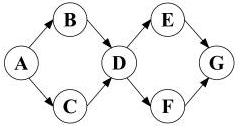
\includegraphics[width=3cm]{figs/nodedisjointb.png}
        \caption{Link-disjoint.}
        \label{Link-disjoint}
    \end{subfigure}
    ~ 
    \begin{subfigure}[t]{0.5\textwidth}
        \centering
        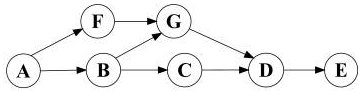
\includegraphics[width=5cm]{figs/nodedisjointc.png}
        \caption{Partially-disjoint.}
        \label{Partially-disjoint}
    \end{subfigure}
    \caption{Categorias de protocolos de múltiplos caminhos, de acordo com o grau de separação dos caminhos. \cite{radi2012multipath}}
\end{figure*}

A seleção dos caminhos ocorre de acordo com a necessidade da aplicação. No caso das \ac{RSSF}s é interessante que os caminhos sejam escolhidos levando em conta o estado da bateria dos módulos que rotearão os pacotes. Porém, pode-se optar por melhorar a confiabilidade da rede. Para isso, os pacotes podem ser transmitidos, de forma redundante, por múltiplos caminhos. Outra possibilidade seria transmitir os dados por apenas um dos caminhos, deixando o restante dos caminhos como \textit{backup} para eventos de falha de módulos ou enlaces.

A manutenção dos caminhos pode ser feita, segundo \citeonline{radi2012multipath}, em um dos seguintes três eventos: (1) Quando um dos caminhos falha, (2) Quando todos os caminhos falham ou, (3) Quando um certo número de caminhos falham. Alguns protocolos classificados como \textit{on-demand} permitem que a manutenção da rede seja realizada em tempo real, através da descoberta e o constante monitoramento dos caminhos. Nessa classificação, existem os \textit{proactive on-demand} que descobrem e mantêm os caminhos ao longo da vida útil da rede, e os \textit{reactive on-demand} que descobrem um novo caminho somente quando necessário, isto é, antes de uma transmissão de dados (\citeonline{Mbarushimana}).

\section{\textit{Redes Definidas por Software (SDN)}}
\label{s_c2_sdn}

As infraestruturas de redes tradicionais são compostas por dispositivos, como roteadores e \textit{switches}, que executam algoritmos complexos e, muitas vezes com interfaces de controle limitadas e específicas do fabricante do equipamento. Consequentemente, a manutenção e atualização dos protocolos da rede (e.g. IPV6), torna-se um desafio \cite{nunes2014survey}. O \ac{SDN} foi projetado para facilitar o gerenciamento das redes de forma flexível e programática. Isto é feito ao retirar a complexidade de controle da rede dos equipamentos (\textit{hardware}) e, repassá-la para uma aplicação controladora, em \textit{software} \cite{Klauberg2016}. 

O principio básico do \ac{SDN} é a separação da rede em planos de controle e dados (Figura \ref{SDN_Arch}). Onde o primeiro é responsável pelas decisões de encaminhamento e o segundo pelo encaminhamento dos dados:

\begin{itemize}
  \item \textbf{\textit{Camada de controle}:} Esta camada é composta por um controlador que possui uma visão geral da rede (Camada de Dados) e capacidade para centralizar toda a inteligência da rede, isto é, gerenciar o roteamento, topologia, segurança, \ac{QoS}, e controlar o consumo energético da rede \cite{Ndiaye}. Desta forma, os módulos da camada inferior enviam requisições, através de uma \ac{API}, para o controlador sempre que uma nova rota é necessária. O controlador, que pode estar em um servidor remoto, responde com a informação necessária para completar a tabela de roteamento do módulo
  \item \textbf{\textit{Camada de dados}:} Os equipamento (\textit{hardware}) que executam uma mesma ou diferentes aplicações são atribuídos à camada de dados. Estes módulos são responsáveis por realizar o sensoriamento da rede e rotear dados de acordo as informações recebidas pelo controlador.
\end{itemize}


\begin{figure}[h!]
    \centering
    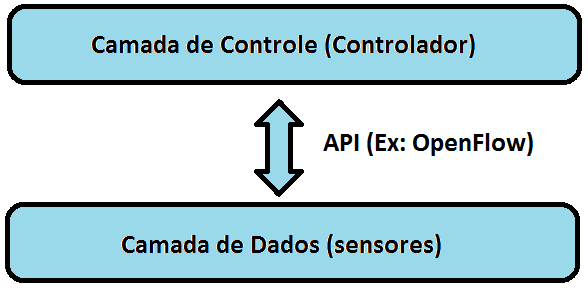
\includegraphics[width=8cm]{figs/sdnArch.png}
    \caption{Arquitetura do \textit{Software Defined Networking}}
    \label{SDN_Arch}
\end{figure}

Ao facilitar a manutenção e entregar a inteligência da rede para o controlador, o \ac{SDN} permite que as exigências de \ac{QoS} sejam constantemente acompanhadas. Isso ocorre pois, o administrador pode gerenciar, configurar e otimizar os recursos da rede, em tempo real, utilizando \textit{softwares} automatizados na implementação do controlador \cite{karakus2017quality}. Além de que, o controlador pode possuir múltiplos algoritmos que atendam às exigências de \ac{QoS} especificas de cada fluxo da rede. Por fim o uso de protocolos como o\textit{OpenFlow}\footnote{\url{https://www.opennetworking.org/technical-communities/areas/specification/open-datapath/}} permite ainda,  o uso de filas para definir diferentes taxas de transmissão para os fluxos da rede.

O \textit{OpenFlow} é a principal \ac{API}, utilizada nas redes SDN, para padronizar a comunicação entre as camadas de controle e dados. Os dispositivos da camada de dados, chamados de \textit{OpenFlow switch}, possuem uma ou mais tabelas de roteamento (\textit{flow table}) e um canal de comunicação segura com o controlador \cite{Klauberg2016}.

 As tabelas de roteamentos são compostas por regras de correspondência, estatísticas e ações. Quando um pacote é recebido, as regras de correspondência são comparadas com informações presentes no cabeçalho, porta de ingresso ou metadado do pacote. Se alguma das regras é validada, então a ação correspondente da \textit{flow table} é disparada. No caso de não haver correspondências, uma regra conhecida como \textit{table-miss} é utilizada para definir o destino do pacote, que pode ser descartado, encaminhado para outra \textit{flow table} ou transmitido para o controlador. Por fim, as informações de estatística incluem dados como número de pacotes e \textit{bytes} recebidos \cite{nunes2014survey}.
 
 O controlador da rede utiliza o canal de comunicação segura, através do protocolo \textit{OpenFlow}, para criar, remover ou modificar regras da \textit{flow table}. O que pode ser feito de maneira reativa (em resposta ao pacote recebido) ou proativa. Já, os \textit{OpenFlow switches} utilizam o canal, no caminho inverso, para requisitar instruções de processamento de um pacote que não possui um regra de correspondência.
 
O \ac{ForCES} é outra \ac{API} que, assim como o \textit{OpenFlow}, prevê a criação das camadas de controle e dados, e padroniza a comunicação entre elas. Criado pela \ac{IETF}, o padrão instancia uma entidade (\ac{FE}) para a camada de dados e outra (\ac{CE}) para a de controle. No \ac{ForCES}, o \ac{FE} possui um bloco (\ac{LFB}) que o controlador utiliza para configurar o \textit{hardware} e definir como os pacotes serão processados \cite{nunes2014survey}. Porém, diferentemente do que ocorre no \textit{OpenFlow}, as camadas de dados e controle continuam coexistindo no mesmo \textit{hardware}. Por esse motivo, esta proposta é menos utilizado na criação de redes SDN, se comparado ao \textit{OpenFlow}. 
 
\section{\ac{SDN} em redes de sensores: SDN-WISE}
\label{s_c2_wise_sdn}

Apesar de atenderem às necessidades de comunicação dos módulos, as \ac{RSSF}s se tornam complexas de gerenciar e configurar a medida que o número de componentes aumenta. Dessa forma, a utilização da arquitetura do \ac{SDN}, é interessante devido à possibilidade de retirar a complexidade do processo de roteamento dos módulos limitados em bateria, processamento e memória e entregá-la para a camada de controle. Além disso, segundo \citeonline{Ndiaye}, o potencial visto no \ac{SDN} se deve à simplificação do gerenciamento e, da reconfiguração da rede devido à existência de um controlador centralizado.  

Aplicações de sensoriamento ambiental, por exemplo, que detectam queimadas, poluição e temperatura podem exigir o uso de centenas ou até milhares de sensores espalhados em ambientes críticos, sem acesso à fontes de energia e com instabilidade climática. Portanto, a viabilidade da aplicação depende da facilidade de configuração, roteamento e manutenção dos dispositivos. Por isso, é evidente que o uso de um controlador centralizado, que possui visão completa da topologia da rede e, capacidade de tomada de decisões para garantir o funcionamento da rede facilita e, viabiliza a criação de amplas redes de sensores sem fio.

\subsection{Visão Geral}

O \ac{SDN} se popularizou graças ao \textit{OpenFlow} que consolidou-se como um dos primeiros protocolos \ac{SDN} à definir uma \ac{API} de comunicação entre Camadas de Controle e Dados. Porém, o \textit{OpenFlow} foi pensado para redes cabeadas e, portanto, não pode ser utilizado para amenizar as dificuldades encontradas no gerenciamento das \ac{RSSF}s em virtude das limitações de \textit{hardware} (memória, bateria e processamento), e da heterogeneidade de dispositivos. 

Assim sendo, em \citeonline{galluccio2015sdn}, os autores se basearam no \textit{OpenFlow} para criar o \ac{SDN-WISE}, que define uma arquitetura \ac{SDN} para \ac{RSSF}s que, permite criar e comunicar controladores da rede, módulos sorvedouros (\textit{Sink}) e fontes (\textit{Source}). O \ac{SDN-WISE}, diferentemente do \textit{OpenFlow}, implementa funcionalidades que melhoram a eficiência energética da rede. Por exemplo, é possível desligar o rádio dos módulos periodicamente (\textit{duty-cycle}), permite-se que os módulos agreguem suas mensagens à pacotes oriundos dos vizinhos, que são roteados através deles. Além do mais, o protocolo \ac{SDN-WISE} prevê que os módulos possuam capacidade de decisão em alguns casos. Dessa forma, diminui-se a quantidade de interações entre os módulos e o controlador e, melhora-se a eficiência energética da rede.

O comportamento esperado dos módulos que compõe uma rede que utiliza o \ac{SDN-WISE} foi descrito em \citeonline{galluccio2015sdn}. Os módulos possuem três estruturas de dados: (i) \textit{WISE States Array}, (ii) \textit{Accepted IDs Array}, e (iii) \textit{WISE Flow Table}, utilizadas para armazenar as informações de roteamento recebidas do controlador da rede. 

O \ac{SDN-WISE} foi projetado para operar em modo \textit{stateful}. Dessa forma, os módulos são projetados como uma máquina de estados, para reagir a um determinado evento de acordo com o estado em que ele se encontra. A vantagem desta abordagem é a redução da quantidade de interações com o controlador, já que o módulo ganha capacidade de reagir à um dado evento com base em informações locais. Para isso o \textit{WISE States Array} é utilizado para armazenar os estados de cada módulo da rede. 

Todos os pacotes transmitidos na rede devem possuir uma \ac{ID} que é utilizada nos módulos receptores para verificar se o pacote deve ser processado ou descartado por eles. Esta verificação é possível pois existe uma lista de \ac{ID}s, chamada de \textit{Accepted IDs Array}, que são comparados ao \ac{ID} recebido no pacote. Se o \ac{ID} recebido combina com um dos \ac{ID}s armazenados, então o receptor processa o pacote de acordo com a instrução repassada pelo controlador. Caso contrário, o pacote é descartado. 

Caso haja a necessidade de processar o pacote, o receptor recorre à \textit{WISE Flow Table} para encontrar uma regra que indique uma ação correspondente, que deve ser tomada para realizar o processamento. Se nenhuma regra for encontrada, então o receptor deve requisitar uma nova regra ao controlador. Portanto, o roteamento no \ac{SDN-WISE} ocorre de acordo com regras de correspondência definidas na \textit{WISE Flow Table}. Quando uma condição definida nas regras de correspondência é atendida, uma ação correspondente é executada e as estatísticas em relação à regra são atualizadas. 

\begin{figure}[h!]
    \centering
    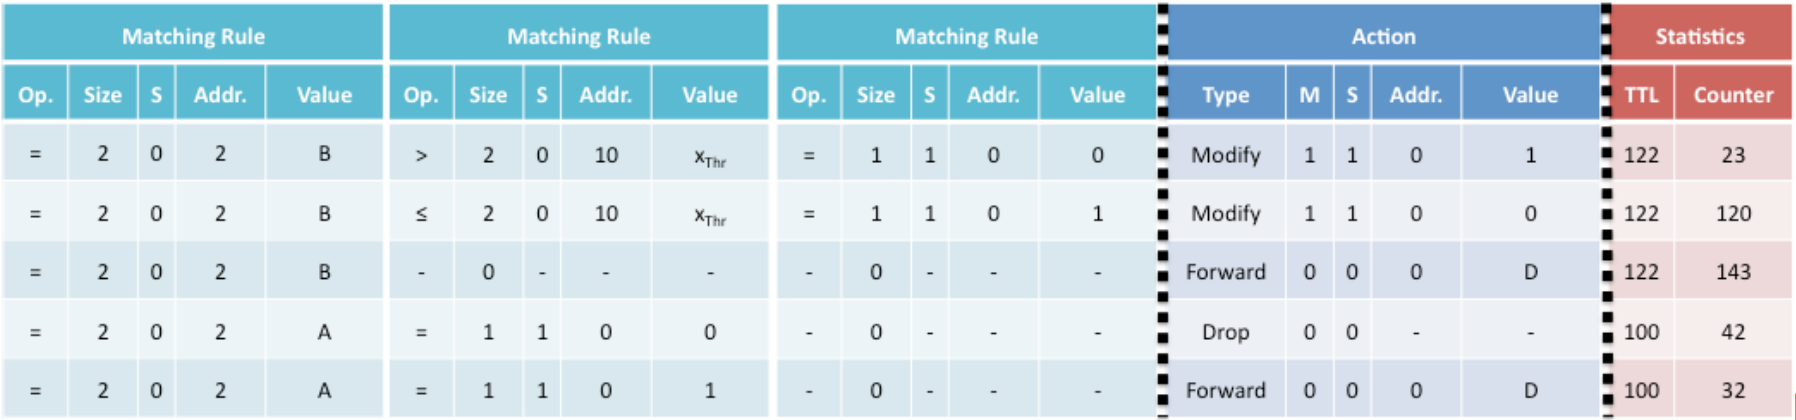
\includegraphics[width=16cm]{figs/WiseFlowTable.png}
    \caption{\textit{WiseFlowTable} \cite{galluccio2015sdn}}
    \label{WiseFlowTable}
\end{figure}

Dessa forma, são definidas três seções na \textit{WISE Flow Table}, como mostrado na Figura \ref{WiseFlowTable}. A primeira seção é a de Regras de Correspondência (\textit{Matching Rules}), que é composta por até três condições (colunas de \textit{Matching Rule}) , que se atendidas, disparam uma ação. O campo S da Regra de Correspondência especifica se a regra é aplicável ao pacote atual ou, ao estado do módulo. Por exemplo, um módulo A que recebe um pacote de B pode executar a ação de acordo com uma informação contida neste pacote ou, com base no estado em que ele se encontra devido à um dado recebido, anteriormente, de um terceiro módulo C. Os campos \textit{Address} e \textit{Size}, indicam respectivamente, o primeiro \textit{byte} e o tamanho da cadeia de caracteres, do pacote ou do estado que devem ser consideradas na regra. O campo \textit{Operator} define o operador relacional a ser utilizado em conjunto com o campo \textit{Value} para verificar se a regra é valida \cite{galluccio2015sdn}.

A segunda seção da \textit{WISE Flow Table} define a ação a ser executada quando as condições da seção Regra de Correspondência são atendidas. O campo \textit{Type} da seção \textit{Action} pode assumir o valor \textit{"Forward to"} para encaminhar, \textit{"Drop"}  para descartar, \textit{"Modify"} para modificar um valor do pacote, \textit{"Send to INPP"} para encaminhar o pacote para a camada \ac{INPP} ou \textit{"Turn off"} para desligar o rádio do módulo. Os campos \textit{Address} e \textit{Size} auxiliam a execução da ação, isto é, complementam a ação indicando, de acordo com o tipo dela, o endereço do módulo para o próximo salto, probabilidade de descarte, onde modificar o pacote ou o estado, o tipo de processamento a ser realizado na \ac{INPP} e o tempo restante até que o rádio seja desligado. O campo S, assim como na seção Regra de Correspondência, indica se a ação é referente ao pacote ou ao estado. E o campo M indica se ação é exclusiva ou não. Ou seja, se outra ação deve ser executada após a atual ou se o processamento deve ser finalizado. 

A terceira seção armazena as estatísticas referentes ao uso das regras de correspondência, que são utilizadas para verificar a validade das regras. O campo \ac{TTL} armazena o tempo restante da validade da regra. E o campo \textit{Counter} indica a quantidade de vezes que a regra foi utilizada.

\subsection{Estrutura dos Pacotes}

Os pacotes (\textit{WISE Packets}) projetados para uso nas \ac{RSSF}s com \ac{SDN-WISE} possuem no mínimo dez \textit{bytes} de comprimento. Os campos do cabeçalho (Figura \ref{WISEPacket}), segundo \citeonline{galluccio2015sdn}, são organizados da seguinte maneira:

\begin{figure}[h!]
    \centering
    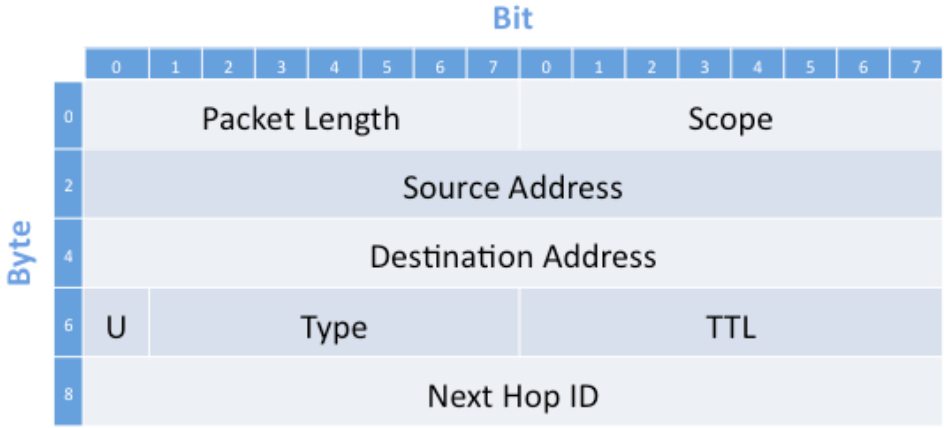
\includegraphics[width=10cm]{figs/WISEPacket.png}
    \caption{Cabeçalho do \textit{Wise Packet} \cite{galluccio2015sdn}}
    \label{WISEPacket}
\end{figure}


\begin{itemize} 
    \item \textbf{\textit{Packet length}:} Indica o tamanho total do pacote (incluindo o \textit{payload}).
    \item \textbf{\textit{Scope}:} Indica um ou mais controladores da rede que têm interesse no pacote.
    \item \textbf{\textit{Source Address} e \textit{Destination Address}:} Indicam o endereço de origem e destino, respectivamente.
    \item \textbf{\textit{Flag U}:} Indica que o pacote deve ser entregue para o \textit{sink} mais próximo.
    \item \textbf{\textit{Type of packet}:} Indica o tipo do pacote e determina como ele será processado pelo receptor. Existem oito tipos de pacotes. Dessa forma, além de dados, o pacote pode carregar informações da topologia da rede, configuração entre módulos e controlador, configuração da \textit{WISE Flow Table} e instruções para desligamento do rádio por um determinado intervalo de tempo.
    \item \textbf{\textit{\ac{TTL}}:} Indica o tempo de vida do pacote e, é decrementado de um a cada salto.
    \item \textbf{\textit{Next Hop ID}:} É o \ac{ID} utilizado pelo receptor para verificar, no \textit{Accepted IDs Array}, se o pacote deve ou não ser processado por ele. 
\end{itemize}

Todos os pacotes transmitidos, internamente, na rede ou para o controlador possuem o mesmo formato do cabeçalho, porém informações distintas no \textit{payload}. A diferença entre eles é destacado no campo \textit{Type} que, como mostrado em \citeonline{sdnwiseCORE}, pode assumir um dos seguintes valores:
\begin{description}
    \item [0]\textbf{\textit{Data}:} Pacote composto apenas pelo cabeçalho e \textit{payload}. 
    \item [1]\textbf{\textit{Beacon}:} Transmitido através de um \textit{broadcast}, o pacote é utilizado para que os módulos compartilhem informações de bateria e distância do \textit{sink}.
    \item [2]\textbf{\textit{Report}:} Utilizado para manter o controlador atualizado sobre o estado dos enlaces na rede. O pacote, transmitido pelos módulos da rede, é composto por informações da vizinhança (endereço e indicador \ac{RSSI}), além da sua distância do \textit{sink} e nível de bateria.   
    \item [3]\textbf{\textit{Request}:} Pacote utilizado para transmitir ao controlador uma requisição de regra de correspondência. Ou seja, a transmissão deste pacote é realizada se, não há uma regra para tratar um pacote recém recebido pelo módulo. Para isso, o módulo encapsula o pacote que não possui regra de correspondência no \textit{payload} da \textit{Request}, e o envia para o controlador. 
    \item [4]\textbf{\textit{Response}:} Pacote, transmitido pelo controlador, que contém a resposta à requisição de uma nova regra de correspondência.
    \item [5]\textbf{\textit{OpenPath }:} Este tipo de pacote tem como finalidade diminuir a quantidade de pacotes transmitidos na rede. Para isso, o controlador cria um caminho de roteamento e transmite, neste pacote, as condições de uso e, os endereços de todos os módulos que compõem o caminho.
    \item [6]\textbf{\textit{Config}:} Utilizado na configuração da rede.
    \item [7]\textbf{\textit{RegProxy}:} Pacote transmitido pelo \textit{sink}, para o controlador, para notificar a sua existência.
\end{description}

\iffalse==============<COMENTADO FORA>==============
\begin{description}
    \item [0]\textbf{\textit{Data}:} Pacote composto apenas pelo cabeçalho e \textit{payload}. 
    \item [1]\textbf{\textit{Beacon}:} Transmitido através de um \textit{broadcast}, o pacote é composto por:
        \begin{itemize} 
            \item \textbf{\textit{Header} - \textit{Bytes} 0-9}: Cabeçalho do \textit{ Wise Packet}.
            \item \textbf{\textit{Distance} - \textit{Byte} 10}: Distância, em saltos, que o módulo está do \textit{sink}.
            \item \textbf{\textit{Battery} - \textit{Byte} 11}: Informação do nível da bateria do módulo. Sendo que, 0xFF é o nível mais alto e 0x00 indica que a bateria está esgotada.
        \end{itemize}
    \item [2]\textbf{\textit{Report}:} Utilizado para manter o controlador atualizado sobre o estado dos enlaces na rede. O pacote é composto por
        \begin{itemize} 
            \item \textbf{\textit{Header} - \textit{Bytes} 0-9}: Cabeçalho do \textit{ Wise Packet}.
            \item \textbf{\textit{Distance} - \textit{Byte} 10}: Distância, em saltos, que o módulo está do \textit{sink}.
            \item \textbf{\textit{Battery} - \textit{Byte} 11}: Informação do nível da bateria do módulo. Sendo que, 0xFF é o nível mais alto e 0x00 indica que a bateria está esgotada.
            \item \textbf{\textit{NeigborsSize} - \textit{Byte} 12}: Indica a quantidade de módulos vizinhos sendo reportados.
            \item \textbf{\textit{NeighborAddress 1} - \textit{Bytes} 13-14}: Endereço do primeiro vizinho da lista.
            \item \textbf{\textit{LinkQuality 1} - \textit{Byte} 15}: indicador \textit{RSSI} de qualidade do enlace entre o módulo e o seu primeiro vizinho da lista.
            \item \textbf{\textit{NeighborAddress n} - \textit{Bytes} ...-... }: Endereço do n-ésimo vizinho da lista.
            \item \textbf{\textit{LinkQuality n} - \textit{Byte} ... }: indicador \textit{RSSI} de qualidade do enlace entre o módulo e o seu n-ésimo vizinho da lista.
        \end{itemize}
    \item [3]\textbf{\textit{Request}:} Pacote utilizado para transmitir ao controlador uma requisição de regra de correspondência. Ou seja, a transmissão é realizada se não há uma regra para tratar um pacote recém recebido pelo módulo. Para isso, o módulo encapsula o pacote que não possui regra de correspondência no \textit{payload} da \textit{Request}, e o envia para o controlador. 
        \begin{itemize} 
            \item \textbf{\textit{Header} - \textit{Bytes} 0-9}: Cabeçalho do \textit{ Wise Packet}.
            \item \textbf{\textit{id} - \textit{Byte} 10}: Identificador da requisição.
            \item \textbf{\textit{Part} - \textit{Byte} 11}: Devido ao encapsulamento do pacote recebido, a \textit{Request} pode ser divida em partes, quando necessário. Portando, este campo identifica qual parte do pacote está sendo transmitido. 
            \item \textbf{\textit{Total} - \textit{Byte} 12}: Indica o número total de parte do pacote.
            \item \textbf{\textit{Unmatched Packet} - \textit{Bytes} 13-14}: Pacote, sem regra de correspondência, recém recebido.
        \end{itemize}
    \item [4]\textbf{\textit{Response}:} Pacote, transmitido pelo controlador, que contém a resposta à requisição de uma nova regra de correspondência.
        \begin{itemize} 
            \item \textbf{\textit{Header} - \textit{Bytes} 0-9}: Cabeçalho do \textit{ Wise Packet}.
            \item \textbf{\textit{Rule} - \textit{Bytes} 10 - ... }: Regra de correspondência.
        \end{itemize}
    \item [5]\textbf{\textit{OpenPath }:} Este tipo de pacote tem como finalidade diminuir a quantidade de pacotes transmitidos na rede. Para isso, o controlador transmite, neste pacote, os endereços de todos os módulos que compõem o caminho e, as condições para o uso caminho.
        \begin{itemize} 
            \item \textbf{\textit{Header} - \textit{Bytes} 0-9}: Cabeçalho do \textit{ Wise Packet}.
            \item \textbf{\textit{WindowSize} - \textit{Byte} 10}: As condições podem ser criadas através de \textit{Windows}, que são compostas por dois valores e um operador relacional. O \textit{Byte} WindowSize indica quantas \textit{Windows} serão criadas.
            \item \textbf{\textit{Window 1} - \textit{Bytes} 11-15}: A primeira \textit{Window} adicionada às regras.
            \item \textbf{\textit{Window n} - \textit{Bytes} ... - ... }: A n-ésima \textit{Window} adicionada às regras.
            \item \textbf{\textit{Address 1} - \textit{Bytes} ... - ...}: O primeiro módulo no caminho.
            \item \textbf{\textit{Address k} - \textit{Bytes} ... - ...}: O k-ésimo módulo no caminho.
        \end{itemize}
    \item [6]\textbf{\textit{Config}:} Utilizado na configuração da rede.
        \begin{itemize} 
            \item \textbf{\textit{Header} - \textit{Bytes} 0-9}: Cabeçalho do \textit{ Wise Packet}.
            \item \textbf{\textit{ConfigId} - \textit{Byte} 10}: Indica o tipo de configuração a ser realizada.
            \item \textbf{\textit{Params} - \textit{Bytes} 11- ... }: Opcional - Indica o valor a ser lido ou escrito.
        \end{itemize}
    \item [7]\textbf{\textit{RegProxy}:} Pacote transmitido pelo \textit{sink}, para o controlador, para notificar a sua existência.
        \begin{itemize} 
            \item \textbf{\textit{Header} - \textit{Bytes} 0-9}: Cabeçalho do \textit{ Wise Packet}.
            \item \textbf{\ac{DPID} - \textit{Bytes} 10-17}: \ac{DPID} do \textit{sink}.
            \item \textbf{\ac{MAC} - \textit{Bytes} 18-23 }: \ac{MAC} do \textit{sink}.
            \item \textbf{\textit{Port} - \textit{Bytes} 24-31 }: Porta física do \textit{sink} .
            \item \textbf{\ac{IP} - \textit{Bytes} 32-35 }: Endereço \ac{IP} do \textit{sink}.
            \item \textbf{\ac{TCP} - \textit{Bytes} 36-37 }: Porta \ac{TCP} do \textit{sink}.
        \end{itemize}
\end{description}
==============</COMENTADO FORA>==============
\fi

\subsection{Camadas de Dados}

Na camada de dados do \ac{SDN-WISE}, os módulos são classificados como sorvedouros (\textit{sink}) e fonte (\textit{source}). A diferença na arquitetura dos dois, como mostrado na Figura \ref{Arq_camada_de_dados}, é que o \textit{sink} possui um módulo de adaptação de dados que serve para adequar o formato dos pacotes ao exigido para comunicação com o controlador da rede. Outras três camadas foram projetadas para os módulos da camada de dados:

\begin{figure}[!htb]
    \centering
    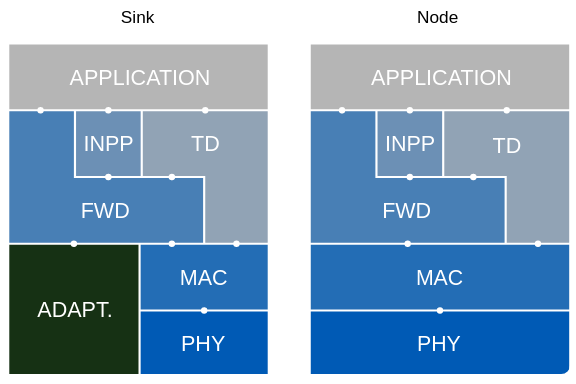
\includegraphics[width=8cm]{figs/arq_camada_de_dados.png}
    \caption{Arquitetura dos módulos \textit{sink} e \textit{source}. \cite{sdnwiseWebSite}}
    \label{Arq_camada_de_dados}
\end{figure}

\begin{itemize} 
  \item \textbf{\textit{In-Network Packet Processing} :} O \ac{INPP} contribui para a eficiência energética do módulo, pois é nesta camada que é realizada a agregação de dados. O módulo pode agregar sua própria mensagem à pacotes que são roteados através dele e que serão entregues à um destino em comum. 
  \item \textbf{\ac{TD}:} A camada \ac{TD} possui um protocolo que coleta informações, geradas pelos módulos, sobre a topologia da rede e às disponibiliza para o controlador. Além do mais, esta camada é responsável por descobrir e manter atualizado o próximo salto de roteamento em direção à um dos \textit{sinks} da rede. Assim, os \textit{sinks} são responsáveis por enviar, periodicamente, pacotes de descoberta de topologia (\textit{TD packet}), através de um \textit{broadcast}, para os módulos \textit{source} da \ac{RSSF}. Neste pacote são enviados o \ac{ID} do \textit{sink}, informação de bateria e um contador, inicialmente zerado, que indica a distância, em saltos, que um módulo está do \textit{sink}.
  
  De acordo com \citeonline{galluccio2015sdn}, o protocolo utilizado no \ac{TD} pode ser descrito em 4 etapas. Supondo que um módulo A recebe um \textit{TD packet} de um módulo B (que pode, ou não, ser um \textit{sink}):
  \begin{enumerate}
    \item O módulo A cria, se já não existe, uma referência para B como um de seus vizinhos. E, armazena as informações de \ac{RSSI} e nível de bateria de B.
    \item O módulo A verifica se já não recebeu um \textit{TD packet} que contenha informação de distância menor. Caso a informação de distância recebida no último pacote seja menor, então uma nova rota, mais rápida, para chegar à um \textit{sink} foi encontrada. Caso contrário o módulo A ignora a informação de distância e apenas incrementa o contador de saltos do pacote.
    \item O módulo A atualiza a informação de bateria do pacote com seu nível de bateria.
    \item O módulo A retransmite o pacote recebido de B.
  \end{enumerate}

Os módulos \textit{source} transmitem, periodicamente, informações sobre a sua vizinhança para o controlador da rede. A taxa de envio dessas informações deve ser escolhida de forma a encontrar um equilíbrio entre manter o controlador atualizado e evitar uma grande quantidade de pacotes na rede (\textit{overhead}). 

    \item \textbf{\ac{FWD}:} O protocolo da camada \ac{FWD} é o responsável por receber os pacotes e realizar o processamento deles de acordo com as informações recebidas no \textit{header} do pacote e, com as disponíveis na \textit{WISE flow table}.
\end{itemize}

\subsection{Exemplo de um cenário simulado}

 O Cooja é uma ferramenta de simulação de rede de sensores sem fio, utilizada para criar cenários compostos por uma \ac{RSSF} e um controlador na nuvem. Desenvolvido para simular e depurar códigos de programas escritos para o sistema operacional Contiki, o Cooja permite emular sensores à nível de \textit{Hardware}. Dessa forma, é possível, através das ferramentas disponibilizadas, verificar a comunicação na rede, por exemplo. Além do mais, é possível acessar a \ac{RSSF} simulada através de portas serial e \ac{TCP}.

Dessa maneira, é possível implementar um controlador que se conecte à rede, através de uma das portas disponibilizadas, e se comunique com um dos \textit{sinks}. O controlador utilizado nas \ac{RSSF}s, que implementam o \ac{SDN-WISE}, pode ser desenvolvidos na linguagem de programação de preferência do administrador da rede. Bastando que o controlador implemente a \ac{API} definida pelo protocolo. Por exemplo, os autores do \ac{SDN-WISE} disponibilizam\footnote{http://sdn-wise.dieei.unict.it/docs/guides/GetStarted.html} um controlador, desenvolvido em Java, que se conecta, através de uma porta \ac{TCP}, à um \textit{sink} executado no Cooja. Ao conectar-se à \ac{RSSF}, o controlador recebe pacotes de \textit{RegProxy}, seguidos por mensagens de \textit{Report} dos \textit{sinks} da rede, que serão tratados e respondidos com pacotes de configuração ou dados.

Além do controlador, foram disponibilizados uma implementação dos módulos \textit{source} e \textit{sink}. O que possibilita a criação de cenários de testes do \ac{SDN-WISE}, utilizando o Cooja. Por exemplo, a Figura \ref{disposicaoModulosSimulation} mostra um cenário em que uma \ac{RSSF} composta por dez módulos \textit{source} e, um \textit{sink}, se comunica com um controlador sendo executado na nuvem. 

\begin{figure}[!htb]
    \centering
    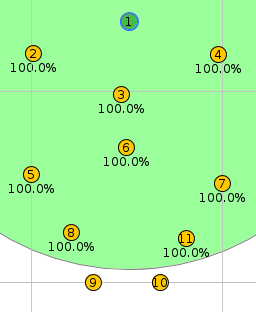
\includegraphics[width=5cm]{figs/disposicaoModulosSimulation.png}
    \caption{Possível cenário de uma \ac{RSSF} executando sobre o \ac{SDN-WISE}.}
    \label{disposicaoModulosSimulation}
\end{figure}

Neste cenário, dez módulos \textit{source} são espalhados em um espaço qualquer, sem interferências. Nota-se que, apenas os módulos identificados com o numeral 9 e 10, estão fora do raio de alcance (área em verde) do \textit{sink}. O que obriga que eles transmitam os seus dados, através de múltiplos saltos até o \textit{sink}. Para isso, o controlador deverá enviar regras de correspondência que serão adicionadas às \textit{WISE Flow Table} de cada um dos módulos. Isto é realizado após a recepção, por parte do controlador, das mensagens de \textit{Report} dos módulos da rede. A reação do controlador é iniciar o seu algoritmo de roteamento para encontrar os melhores caminhos na rede que, neste caso, serão aqueles com menor número de saltos e, portanto menor custo, de acordo com o algoritmo de Dijkstra. Ao fim da execução, o novo caminho de roteamento, é transmitido para a rede utilizando os pacotes de \textit{Response} ou de \textit{OpenPath}.

O Cooja oferece ferramentas que possibilitam depurar, em tempo real, as Regras de Correspondências enviadas  do controlador para os módulos da rede. Por exemplo, na Figura \ref{DescobertaDeCaminhoExemploa}, é possível observar que, o controlador conclui que a melhor forma de rotear pacotes do módulo 10 para \textit{sink} e vice versa, é através do módulo 4. Logo, o módulo 1 insere uma regra em sua \textit{WISE Flow Table} que define o roteamento para o módulo 10, através de 4 e, o módulo 10 recebe uma regra com o caminho inverso.

\begin{figure}[!htb]
    \centering
    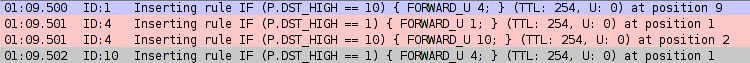
\includegraphics[width=15cm]{figs/regrasDeRoteamentoAtravesDe4.png}
    \caption{Regra de roteamento através do módulo 4.}
    \label{DescobertaDeCaminhoExemploa}
\end{figure}



\section{\ac{QoS} em \ac{RSSF}s com \ac{SDN-WISE}}
\label{s_c2_wise_sdn_QOS}

Uma das diferenças a ser destacada no \ac{SDN-WISE}, em relação ao \textit{OpenFlow}, é a sua capacidade de armazenar estados. Como já mencionado, reagir à recepção de um pacote de acordo com o estado do receptor, diminui o número necessário de comunicações entre módulo e controlador. O que afeta, positivamente, a eficiência energética da rede. Ademais, como demonstrado em \citeonline{di2016exploiting}, os estados podem ser utilizados para representar o congestionamento percebido pelo módulo e, portanto auxiliar na garantia de \ac{QoS} da rede. 

A ideia proposta em \citeonline{di2016exploiting} é utilizar o tamanho da fila do \textit{buffer} de recepção, no qual os pacotes são enfileirados até que sejam processados, para definir os estados do módulo. Por exemplo, um módulo que esteja com sua fila vazia, deve manter-se em um estado inicial \textit{Green} (G). Já quando a fila está cheia, o estado deve ser modificado para \textit{Red} (R) e, o roteamento deve ser alterado para evitar perda de pacotes. Para isso, o controlador cria regras de roteamento com base no congestionamento percebido pelo módulo e, na categorização dos fluxos da rede, em k classes com prioridades distintas, onde $C_1$ possui a mais baixa prioridade e $C_K$, a mais alta. Desta maneira, é possível a diferenciar a forma como os fluxos são tratados e, oferecer garantias de entrega dos pacotes transmitidos. 

O mecanismo apresentado propõe o descarte de pacotes e balanceamento do tráfego da rede. No primeiro caso, é utilizada uma probabilidade menor de descarte dos pacotes oriundos de fluxos com prioridade alta, em detrimento daqueles com menor prioridade. De forma a garantir mais recursos da rede para os fluxos mais criticos, ou seja, com maior prioridade. E no segundo caso, o controlador deve sugerir caminhos alternativos ou múltiplos caminhos para evitar o ponto de congestionamento da rede.

\begin{figure}[!htb]
    \centering
    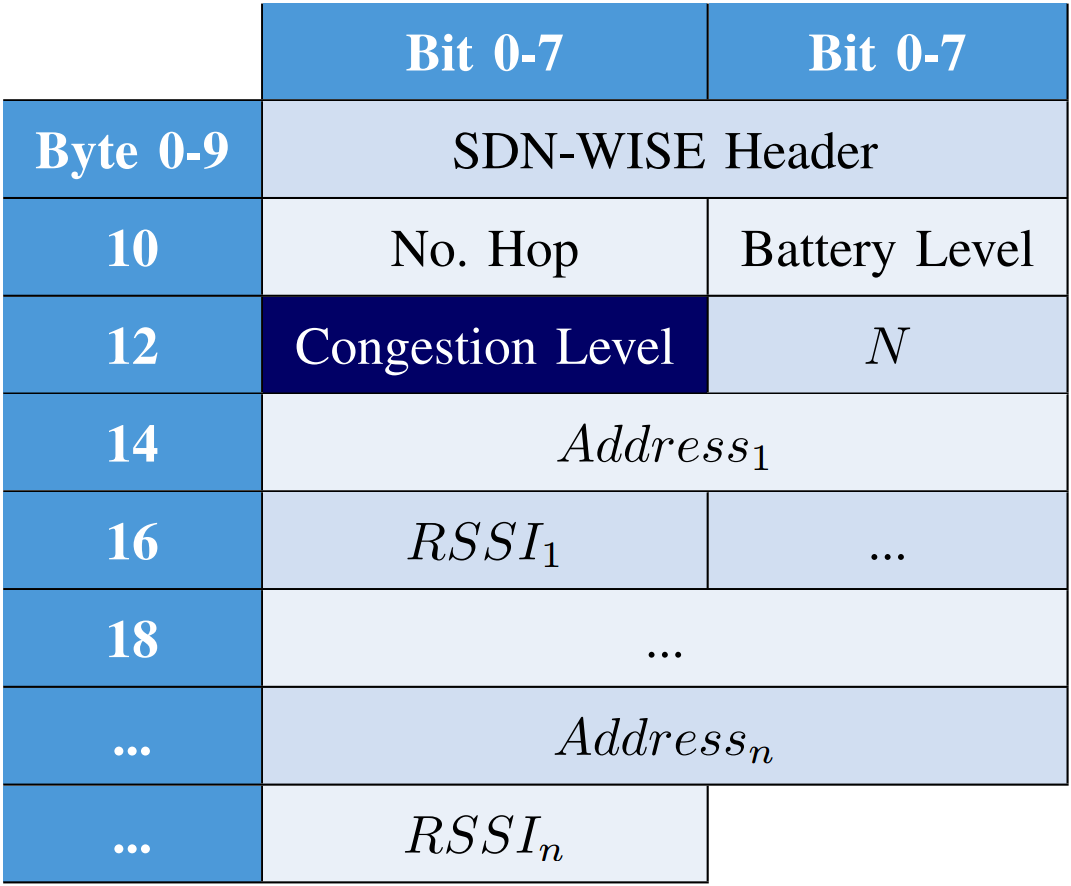
\includegraphics[width=5cm]{figs/NewReport.png}
    \caption{novo pacote SDN-WISE report. \cite{di2016exploiting}}
    \label{NewReport}
\end{figure}

Para integrar essa solução de \ac{QoS} ao \ac{SDN-WISE}, é proposto, ainda em \citeonline{di2016exploiting}, que um campo \textit{Congestion Level} seja adicionado ao pacote \textit{Report}, como mostrado na Figura \ref{NewReport}. E que, três estados, cujas transições ocorrem de acordo com o tamanho da fila no \textit{buffer} de recepção, sejam utilizados para determinar como um pacote deve ser processado:

  \begin{enumerate}
    \item \textbf{\textit{Green} (G):} Representa o estado inicial da fila, em que ela está vazia. Ou seja, não há congestionamento na rede e, portanto não há descarte de pacotes ou necessidade de caminhos alternativos. A transição para o próximo estado ocorrerá somente quando a fila alcançar o limite definido por $T_{GY}$.
    \item \textbf{\textit{Yellow} (Y):} Representa o estado em que há pacotes em espera na fila. Porém, o tamanho da fila ainda não atingiu o limite máximo, definido por $T_{YR}$. Neste estado, o módulo receptor passa a descartar pacotes com uma certa probabilidade, repassada pelo controlador, de acordo com a prioridade do fluxo. Isso é feito com objetivo de garantir a entrega dos pacotes oriundos de fluxos com alta prioridade. 
    \item \textbf{\textit{Red} (R):} Representa o estado em que a fila está cheia. Neste caso, a probabilidade de descarte dos pacotes oriundos de fluxos de baixa prioridade é ainda maior que o repassado, pelo controlador, para o estado Y.
  \end{enumerate}

Um possível cenário de uso para a abordagem proposta em \citeonline{di2016exploiting}, é mostrado na Figura \ref{cenarioExemploSDNWISE_QOS}. Onde em um primeiro momento T1, apenas os módulos do tipo A, transmitem seus pacotes para o \textit{sink}. Estes pacotes têm prioridade $C_3$ e são roteados através do módulo 1, que está no estado G. Em um segundo momento T2, o módulo do tipo B inicia sua transmissão utilizando um fluxo com prioridade $C_1$, o que faz com que o limite $T_{GY}$ do módulo 1 seja atingido, e o estado seja alterado para Y.

\begin{figure}[!htb]
    \centering
    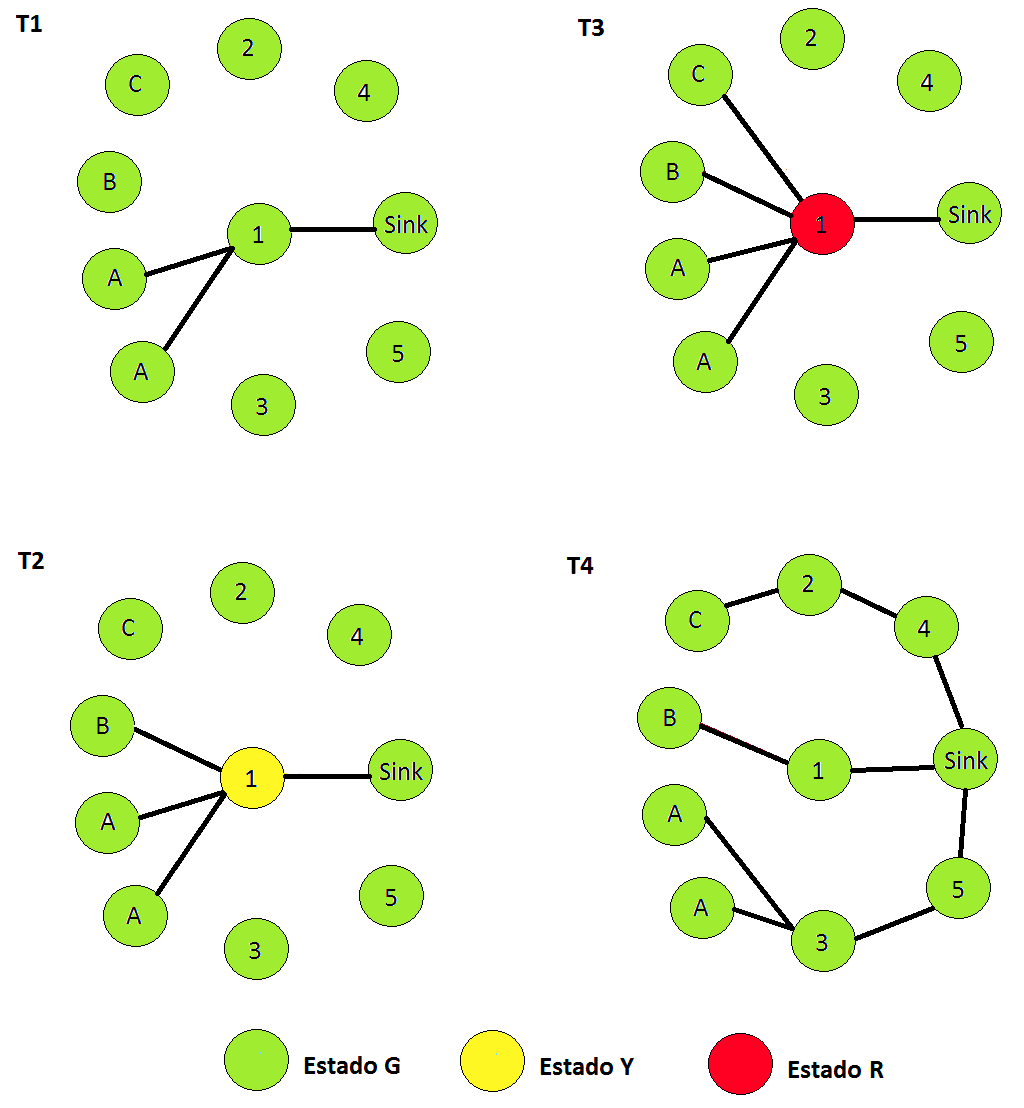
\includegraphics[width=8cm]{figs/novocenarioExemploSDNWISE_QOS.png}
    \caption{Possível cenário de congestionamento e garantia de \ac{QoS} utilizando SDN-WISE.}
    \label{cenarioExemploSDNWISE_QOS}
\end{figure}


Como mostrado na Figura \ref{drop_prob}, a partir desse momento a probabilidade de descarte dos pacotes transmitidos dos módulos A passa de 0\% para 5\%. Já, os pacotes do módulo B que, têm a mais alta prioridade, são descartados com probabilidade de 1\%. Em um terceiro momento T3, o módulo C inicia sua transmissão com prioridade $C_2$, o que faz com que o módulo 1 fique completamente congestionado e, transite seu estado para R. Com isso, as probabilidades de descarte aumentam para todas as classes de fluxos, sendo que na \textit{Option 2}, o descarte dos pacotes pode chegar a 80\% para os fluxos com baixa prioridade. Porém, mesmo neste cenário mais critico, os fluxos com alta prioridade possuem garantia de tráfego.

A transmissão, periódica, dos estados dos módulos para o controlador, permite que o roteamento seja realizado dinamicamente. Dessa forma, diante do cenário apresentado em T3, o controlador pode, por exemplo, definir que os fluxos com prioridade $C_3$ sejam desviados para um caminho alternativo. O mesmo pode ser feito para os fluxos com prioridade $C_2$. Resultando na reserva do melhor caminho, escolhido originalmente, para o fluxo do módulo B, que possui prioridade $C_1$, como mostrado na Figura \ref{cenarioExemploSDNWISE_QOS} - T4.

\begin{figure}[!htb]
    \centering
    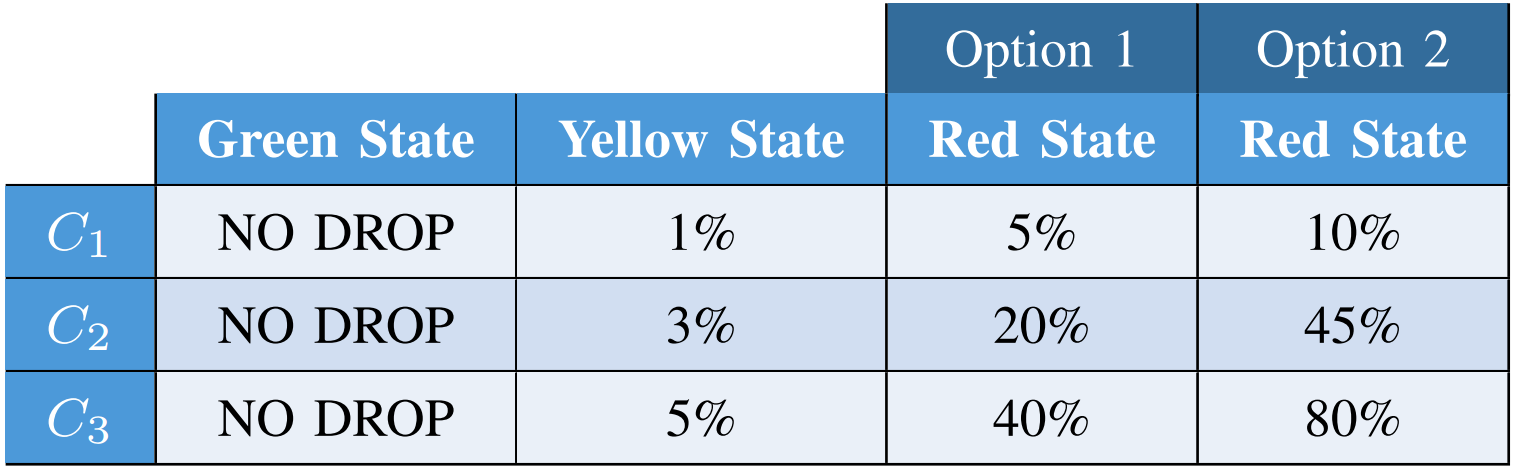
\includegraphics[width=8cm]{figs/drop_prob.png}
    \caption{Probabilidades de descarte de pacotes de acordo com a classe do fluxo. \cite{di2016exploiting} }
    \label{drop_prob}
\end{figure}
% ----------------------------------------------------------------------- %
% Arquivo: cap2.tex
% ----------------------------------------------------------------------- %
\iffalse
==============<COMENTADO FORA>==============


\adESS{Conforme referenciado no Capítulo 1 o objetivo geral deste trabalho é implementar uma rede de sensores sem fio, baseada no conceito de SDN (Redes Definidas por Software) com fins de prover QoS para aplicações que se executam sobre a RSSF.}

\adESS{Um dos resultados esperados do mesmo é ganhar experiência com a aplicação de SDN em redes de Sensores e verificar as potencialidades de explorar este conceito em aplicações com requisitos de QoS. A plataforma SDN-WISE se apresenta como uma forma adequada para esta finalidade. Desta forma, inicialmente pretende-se implantar e analisar o comportamento de uma aplicação sobre a plataforma SDN-WISE no simulador Cooja e nos sensores Micaz. Embora já exista exemplos sobre o Cooja, a operacionalidade do mesmo sobre nodos reais deve ser avaliada.}


\adESS{Em um segundo momento, pretende-se conceber e implementar um controlador SDN que permita construir regras a partir de uma configuração estática de nodos e fluxos com requisitos de QoS associados a vazão e ao nível de bateria dos nodos.}


\adESS{A Figura \ref{modeloproposto} a seguir esboça uma primeira ideia desta estrutura:}

\begin{figure}[!htb]
    \centering
    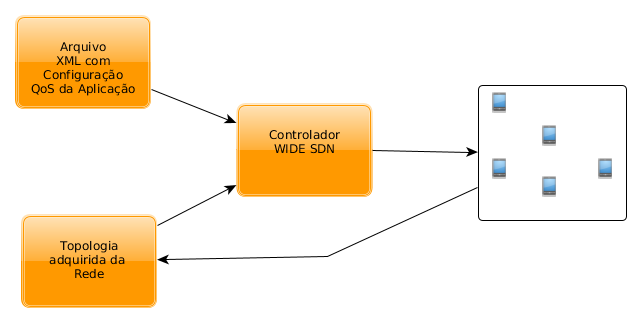
\includegraphics[width=13cm]{figs/DiagramaTCCAndre.png}
    \caption{Um Controlador direcionado a QoS}
    \label{modeloproposto}
\end{figure}

\adESS{Pretende-se conceber um controlador que, através de uma especificação em XML de uma aplicação, através de fluxos gerados em direção a um sorvedouro, e tendo como referência a topologia adquirida pelo SDN-WISE, forneça as regras de roteamento para a rede.}

\adESS{Neste ponto, também pretende-se avaliar a possibilidade de utilizar a visão \textit{statefull} proposta pelo SDN-WISE para ajustar o funcionamento do roteamento sem a necessidade de intervenção constante do Controlador.}

\adESS{Neste TCC não se terá inicialmente a preocupação de produzir um algoritmo ótimo para esta tarefa. O foco será em estabelecer a rede tendo como requisitos de banda e focando também o consumo de energia dos nodos. Como um dos problemas fundamentais em redes de sensores é a questão energética, pretende-se propor regras de roteamento que proporcionem a maximização da vida dos nodos ao mesmo tempo que garantam a banda na transmissão de fluxos que partem de nodos em direção aos sorvedouros.}

\adESS{Deve ser observado que o SDN-WISE permite capturar a topologia da rede, trazendo informações de vizinhos, SNRI e de nível de bateria de nodos. A questão de alocação de fluxos nos caminhos possíveis da rede exigirá um trabalho adicional de avaliação de banda disponível nos enlaces. Em adição, os nodos permitem ajustar a potência de transmissão. Tecnicamente é possível alterar as condições de conectividade da rede em função deste parâmetro. Uma fase de ajuste destas topologia usando esta possibilidade pode ser considerada.}

\adESS{Como continuidade desta etapa, pretende-se investigar a possibilidade de utilização da SDN no roteamento com múltiplos caminhos. Neste sentido, a ideia inicial é dispersar os fluxos através de caminhos disjuntos, expĺorando o roteamento multicaminho e reduzindo o esforço dos nodos em tempos de trabalho. Os requisitos de banda associados aos fluxos deverão ser cumpridos.}

\adESS{Novamente a preocupação aqui não é a confecção de algoritmos ótimos de roteamento, mas sim analisar a viabilidade do uso do sistema explorando regras que possibilitem o comportamento desejado e verificando possíveis problemas associados a esta abordagem.}

==============</COMENTADO FORA>==============
\fi

\chapter{Proposta}
\label{c_cap3}

%O presente trabalho propõe a implementação de uma rede de sensores sem fio, baseada no conceito de \ac{SDN}  para aplicações com requisitos \ac{QoS} que se executam sobre os nodos. Na sequência, a proposta é apresentada com mais detalhes e é apresentado um cronograma de execução.

As limitações de \textit{hardware} dos módulos das \ac{RSSF}s tornam o gerenciamento e a consequente garantia de \ac{QoS}, um desafio para os administradores da rede. Por isso, conforme referenciado no Capítulo \ref{c_introducao}, o objetivo geral deste trabalho é implementar uma rede de sensores sem fio, baseada no conceito de \ac{SDN} com fins de prover \ac{QoS} para aplicações que se executam sobre a \ac{RSSF}.

Para isso, o sistema \ac{SDN-WISE} será utilizado na comunicação entre as camadas da arquitetura \ac{SDN}. Na camada de dados, módulos MICAz que serão, em um primeiro momento, emulados no Cooja e, em seguida utilizados em um cenário real, ficam responsáveis por gerar e rotear os dados da rede. E na camada de controle, um algoritmo de roteamento será utilizado para oferecer garantias de vazão e baixo consumo energético para os módulos da camada de dados. Para tanto, o controlador terá acesso às informações dos módulos, da topologia da rede e dos requisitos de \ac{QoS} da aplicação, por conseguinte, o controlador aplicará as regras de roteamento, dinamicamente, na \ac{RSSF}.

\section{Detalhamento da proposta}

Para cumprir com os objetivos propostos, o trabalho será dividido em etapas de implantação de uma \ac{RSSF} baseada no conceito de \ac{SDN}. A primeira etapa tem como objetivo ganhar experiência com o protocolo \ac{SDN-WISE} e, implantar uma \ac{RSSF} com módulos MICAz. Para isso, a ferramenta de simulação de redes Cooja e módulos MICAz reais, serão utilizados para executar uma aplicação concebida para o trabalho. Já na segunda etapa, pretende-se verificar o potencial do conceito de \ac{SDN} em aplicações com requisitos de \ac{QoS}.

O Cooja permite simular os módulos MICAz, e utilizar o mesmo código (em linguagem C) desenvolvido para os módulos físicos no ambiente de simulação. Além do mais, o Cooja disponibiliza várias ferramentas que auxiliam na depuração do código e na criação de cenários com grande quantidades de módulos. A Figura \ref{simuladorCooja}, mostra algumas das principais ferramentas. A \textit{Network} permite a visualização da troca de pacotes e, o posicionamento dos módulos, de forma gráfica. Já as ferramentas \textit{Mote Output} e \textit{Radio messages}, registram, respectivamente, os \textit{logs} publicados pelos módulos e as mensagens transmitidas através dos seus rádios. Na \textit{Timeline}, é possível observar as transmissões realizadas. Por fim, o Cooja oferece uma interface \ac{TCP} que, pode ser acessada, através de um terminal externo. O que, neste trabalho, permite a integração do controlador com os módulos simulados. Por estas razões, escolheu-se trabalhar com esta ferramenta para implantar uma \ac{RSSF}, baseado no conceito de \ac{SDN}.

\begin{figure}[!htb]
    \centering
    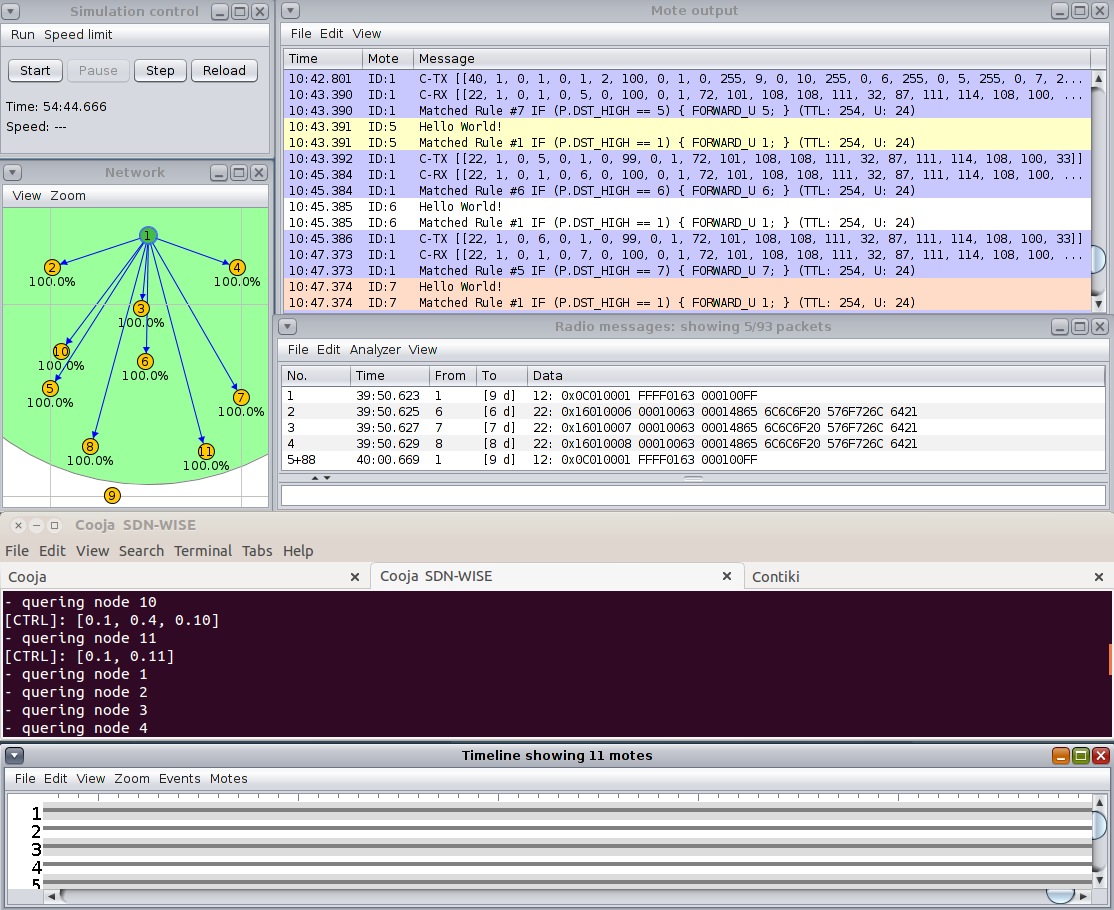
\includegraphics[width=15cm]{figs/simuladorCooja.png}
    \caption{Visão geral do simulador de redes Cooja.}
    \label{simuladorCooja}
\end{figure}

Dessa forma, na primeira etapa, será utilizado um experimento básico, disponibilizado pelos autores do \ac{SDN-WISE} para o Cooja. Neste exemplo, um controlador, desenvolvido em Java, utiliza o algoritmo de Dijkstra para encontrar os caminhos com menor custo. Os módulos (\textit{sink} e \textit{source}), também desenvolvidos em Java, utilizam os caminhos recebidos pelo controlador para rotear os pacotes, gerados de forma aleatória, até o único \textit{sink} da rede. Em seguida, ainda na primeira etapa, pretende-se implantar e analisar o comportamento de uma aplicação sobre a plataforma \ac{SDN-WISE} no Cooja, utilizando sensores MICAz emulados. Embora já exista o exemplo disponibilizado, a operacionalidade do mesmo sobre módulos MICAz deve ser avaliada, uma vez que os módulos (\textit{sink} e \textit{source}) disponibilizados, são genéricos, ou seja, não foram projetados de acordo com as características de \textit{hardware} do MICAz. 

O foco da segunda etapa de desenvolvimento é explorar o conceito de \ac{SDN} em aplicações com requisitos de \ac{QoS}. Para isso, o controlador utilizado na primeira etapa deverá ser modificado. A ideia é que ele possibilite a configuração estática dos módulos e, dos fluxos que possuem requisitos de \ac{QoS} associados à vazão e, ao nível de bateria dos nodos. Além disso, o algoritmo de Dijkstra, padrão do controlador, será substituído por um que faça a alocação de fluxos a caminhos da rede de forma a atender aos requisitos de vazão e consumo energético da aplicação. 

Além das modificações no controlador, outra medidas podem ser implementadas com objetivo de garantir eficiência energética e a largura de banda exigida pela aplicação da rede \ac{SDN}. Por exemplo, pretende-se verificar a possibilidade do uso dos estados, propostos pelo \ac{SDN-WISE}, para alterar o roteamento, sem a necessidade de intervenção constante do controlador e, garantir o tráfego de dados na rede, como mostrado na Seção \ref{s_c2_wise_sdn_QOS}. Pode-se, ainda, utilizar a capacidade, do \ac{SDN-WISE}, de ajuste da potência de transmissão dos módulos, para modificar a topologia da rede, uma vez que, a alteração deste parâmetro impacta diretamente nas condições de conectividade da rede.

Para esta etapa, planeja-se também, verificar a melhor forma de avaliação da largura de banda disponível para cada enlace e, como alocar caminhos com banda disponível para fluxos com exigências de \ac{QoS}. Por fim, pretende-se investigar a possibilidade do uso de algoritmos de roteamento por múltiplos caminhos em \ac{RSSF}s baseadas no conceito de \ac{SDN}. Neste sentido, a ideia inicial é dispersar os fluxos através de caminhos disjuntos, explorando o roteamento multicaminho e reduzindo o esforço dos nodos em tempos de trabalho. 

Assim, pretende-se, ao fim deste trabalho, apresentar a estrutura mostrada na Figura \ref{Arch_wiseSDN_TCC}. A partir dela observa-se que o controlador utiliza as configurações recebidas, através de um arquivo \ac{XML}, em conjunto com informações dos módulos e da topologia da rede para criar regras de roteamento. É importante mencionar que, o foco deste trabalho não é propor um algoritmo ótimo para garantia de \ac{QoS} em aplicações da \ac{RSSF}. Mas sim, analisar a viabilidade do uso do conceito de \ac{SDN}, para atender aos requisitos de \ac{QoS} das aplicações das \ac{RSSF}s e, explorar regras de roteamento, que garantam a maximização da vida dos nodos, ao mesmo tempo que garantam a banda na transmissão de fluxos que, partem de nodos em direção aos sorvedouros da rede.


\begin{figure}[!htb]
    \centering
    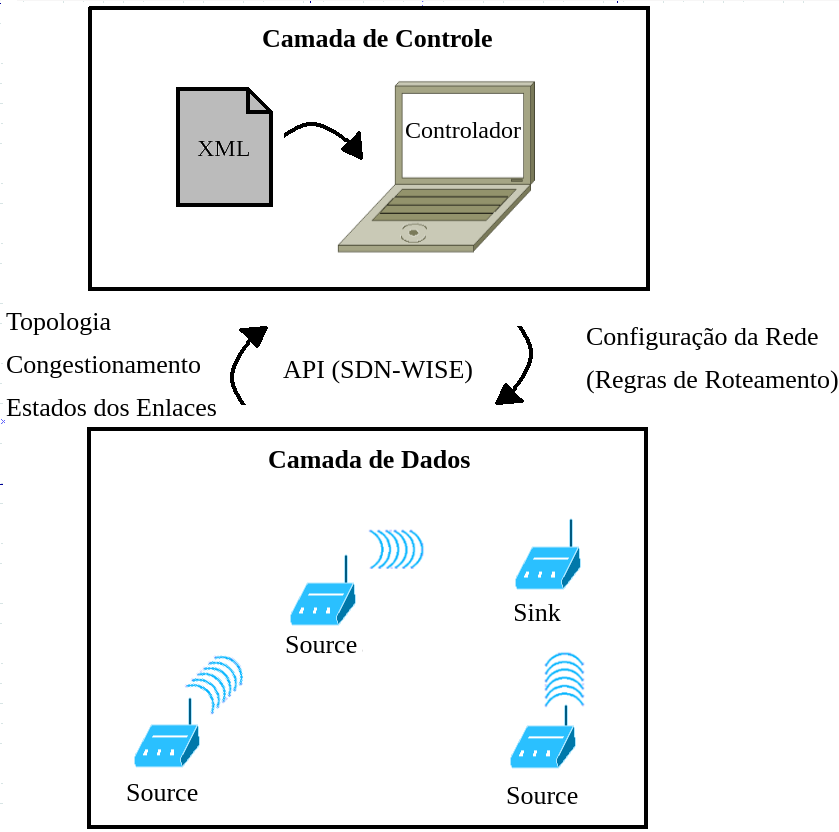
\includegraphics[width=6cm]{figs/Arch_wiseSDN_TCC.png}
    \caption{Arquitetura \ac{SDN} na \ac{RSSF} para garantia de \ac{QoS}}
    \label{Arch_wiseSDN_TCC}
\end{figure}

\section{Recursos, Etapas e Cronograma}

\subsection{Recursos necessários}

\begin{figure*}[t!]
    \centering
    \begin{subfigure}[t]{0.45\textwidth}
        \centering
        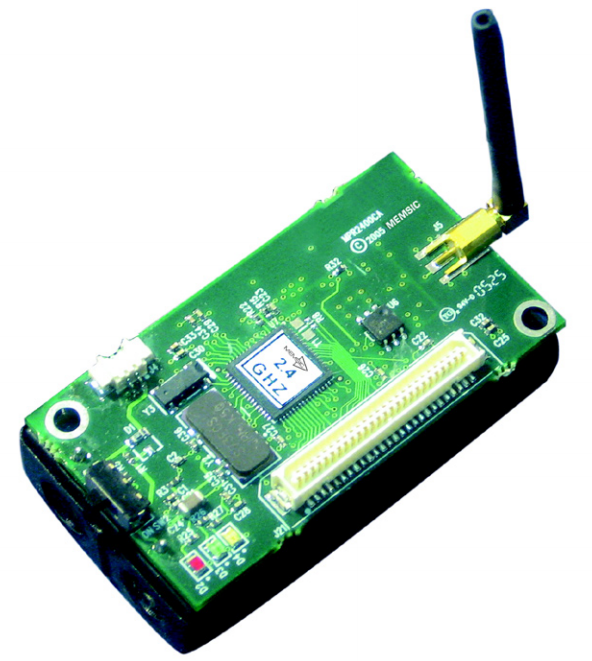
\includegraphics[width=4cm]{figs/ModulosMICAZ.png}
        \caption{Mote MICAz. \cite{micaz2013wireless}}
        \label{ModulosMICAZ}
    \end{subfigure}%
    ~ 
    \begin{subfigure}[t]{0.45\textwidth}
        \centering
        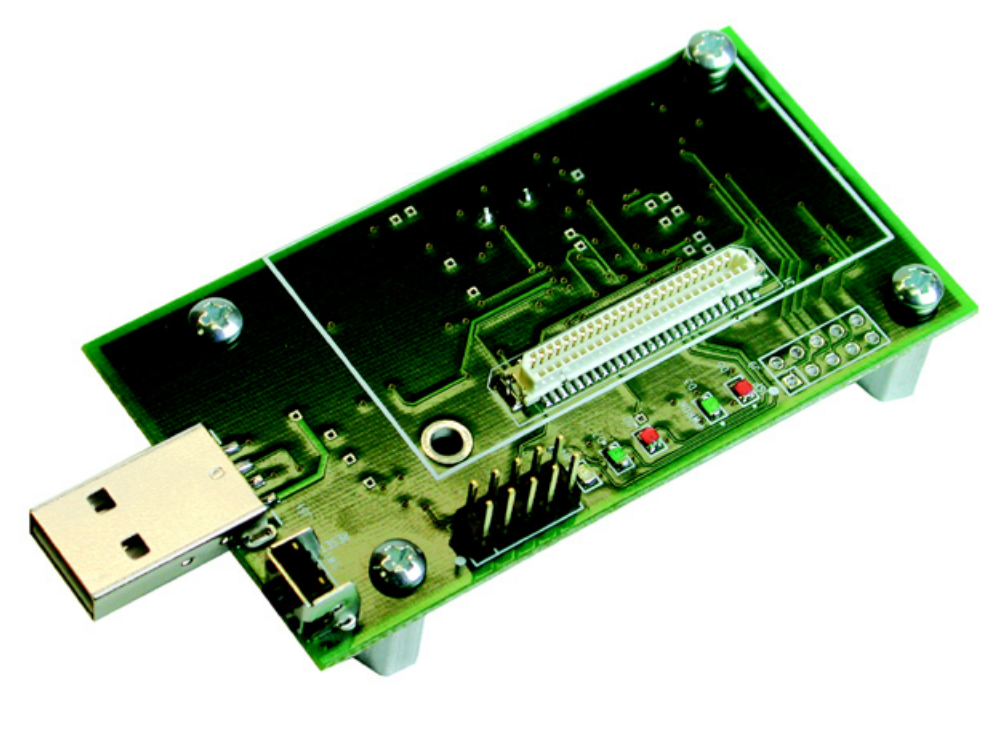
\includegraphics[width=4cm]{figs/InterfaceMICAZ.png}
        \caption{Interface de programação para MICAz. \cite{micaz2013wireless}}
        \label{InterfaceMICAZ}
    \end{subfigure}
    \caption{MICAz e programadora necessária para o trabalho.}
\end{figure*}

O controlador da arquitetura \ac{SDN}, será executado em um \textit{laptop}, e os módulos \textit{sink} e \textit{source} serão implementados com módulos MICAz (Figura \ref{ModulosMICAZ}). Porém, o \textit{sink} será conectado ao \textit{laptop} através da sua interface de programação (Figura \ref{InterfaceMICAZ})


\subsection{Etapas de desenvolvimento}
\begin{itemize}  
    \item Implantação, no Cooja, de uma \ac{RSSF} com arquitetura \ac{SDN}, utilizando o controlador e, módulos \textit{sink} e \textit{source} disponibilizados pelos autores do \ac{SDN-WISE}.
    \item Migração do código dos módulos genéricos para a plataforma MICAz.
    \item Estudo e implementação de uma aplicação piloto.
    \item Análise e implementação de algoritmos de roteamento para \ac{RSSF}s que, ofereçam garantia de vazão e/ou eficiência energética, para a aplicação piloto.
    \item Criar um cenário real com módulo MICAz físicos.
    \item Avaliação do comportamento da \ac{RSSF} implantada no cenário real. 
\end{itemize}

\subsection{Cronograma}

O cronograma mostrado na Tabela \ref{t_cronograma} será seguido, com o objetivo de implantar uma \ac{RSSF}, baseada no \ac{SDN-WISE} para provimento de \ac{QoS}. Cada etapa de desenvolvimento descrita anteriormente será realizada, em pelo menos, duas semanas. Porém, será realizado o acompanhamento semanal, de acordo com abordagens de gestão, como o Kanban. Como visto na tabela, exceto pela escrita e correção do texto, todas as etapas devem ser feitas separadamente, e na sequência que garanta a implementação da etapa seguinte.


\begin{table}[!htpb]
\centering
\begin{small}
  \setlength{\tabcolsep}{3pt}
\begin{tabular}{|c|c|c|c|c|c|c|c|c|c|c|c|c|}\hline
 & \multicolumn{12}{c|}{Mês/Semanas}\\ \cline{2-13}
\raisebox{1.5ex}{Etapa} & Jul & Jul & Ago & Ago & Set & Set & Out & Out & Nov & Nov & Dez & Dez \\ 
                        & 1-2 & 3-4 & 1-2 & 3-4 & 1-2 & 3-4 & 1-2 & 3-4 & 1-2 & 3-4 & 1-2 & 3-4 \\\hline

% exemplo de linha
% 1 & & & & & & & & & & & & \\ \hline

Implantação no Cooja      & X & & & & & & & & & & & \\ \hline
Migração para o MICAz     & & X & X & & & & & & & & & \\ \hline
Aplicação Piloto          & & & & X & & & & & & & & \\ \hline
Algoritmos                & & & & & X & X & & & & & & \\ \hline
Escrita do TCC2           & & & X & X & X & X &  & & & & &  \\ \hline
Cenário Real              & & & & & & & X & X & X & & &  \\ \hline
Avaliação                 & & & & & & & & & & X & &  \\ \hline
Correções do Texto        & & & & & & & X & X & X & X & &  \\ \hline
Entrega da Monografia     & & & & & & & & & & & X &  \\ \hline
Apresentação à banca      & & & & & & & & & & & X &  \\ \hline
Correções e Entrega Final & & & & & & & & & & & & X \\ \hline

\end{tabular} 
\end{small}
\caption{Cronograma das atividades previstas}
\label{t_cronograma}
\end{table} 

\cleardoublepage


% ----------------------------------------------------------
% ELEMENTOS PÓS-TEXTUAIS
% ----------------------------------------------------------
\postextual
% ----------------------------------------------------------

% ----------------------------------------------------------
% Referências bibliográficas
% ----------------------------------------------------------
\bibliography{referencias}


%---------------------------------------------------------------------
% INDICE REMISSIVO
%---------------------------------------------------------------------
\phantompart
\printindex
%---------------------------------------------------------------------

\end{document}
